\documentclass[11pt,a4paper]{article}
\usepackage[utf8]{inputenc}
\usepackage[T1]{fontenc}
\usepackage{amsmath,amssymb,amsfonts}
\usepackage{graphicx}
\usepackage{geometry}
\usepackage{booktabs}
\usepackage{hyperref}

\geometry{margin=2.1cm}
\hypersetup{
    colorlinks=true,
    linkcolor=blue,
    citecolor=blue,
    urlcolor=blue
}
\renewcommand{\figurename}{Ábra}
\renewcommand{\tablename}{Táblázat}
\renewcommand{\refname}{Irodalomjegyzék}
\renewcommand{\contentsname}{Tartalomjegyzék}
\renewcommand{\abstractname}{Összefoglaló (Abstract)}

\title{\textbf{A kozmikus idő-tájkép ($M_\tau^\star$) és az ESA Euclid DR1-Foundation háromdimenziós validációja:}\\
\large Galaxisok közötti óraráta-gradiensek, fekete lyuk--kozmosz idő-dualitás és a sötét szektor $k=0$ paraméteres feloldása 18\,983 élő archívumi objektumon}
\author{Tau Core Kutatási Program (Paper 20 -- Empirikus / Protokoll \& Szintézis Sorozat)}
\date{2026. november 14.}

\begin{document}
\maketitle

\begin{abstract}
A standard $\Lambda\mathrm{CDM}$ kozmológia a világegyetem lokális órarátájának térbeli változékonyságát másodrendű perturbációként ($\Phi/c^2 \sim 10^{-5}$) kezeli egy globálisan szinkronizált Friedmann--Lema\^{\i}tre--Robertson--Walker (FLRW) háttéridő felett, és a galaxisok lapos rotációs görbéit, az erős gravitációs lencsézést, valamint az integrált Sachs--Wolfe (ISW) anomáliákat egy $95\%$-os sötét szektor ($\Omega_{\mathrm{DM}} + \Omega_\Lambda$) bevezetésével magyarázza. Bár a makroszkopikus visszahatás-modellek -- különösen Wiltshire \emph{Timescape} kozmológiája (2007) -- felvetették, hogy a kozmikus ürességek (voidok) és a galaktikus falak órái eltérő ütemben ketyegnek, a Timescape keretrendszer szigorúan a klasszikus általános relativitáselméleten (GR) belül marad: nem rendelkezik mikroszkopikus óramezős határérték-egyenlettel (BVP), szabad elméleti illesztőparamétereket használ ($f_{v0}, \Omega_{M0}$), és nem képes levezetni sem a galaxisok $a_0$ gyorsulási skáláját, sem a halmazok lencsézési tömegét sötét anyag nélkül. Ebben a tanulmányban (Paper 20) bemutatjuk az első teljes, megfigyelés-vezérelt háromdimenziós Tau Core Univerzum Modellt és Idő-Tájkép Atlaszt ($M_\tau^\star$), és zéró szabad végponti paraméterrel ($k=0$) validáljuk azt az ESA Euclid űrtávcső 2026. október 21-én megnyitott DR1-Foundation adattárából (\texttt{esac.esa.int/tap-server/tap}, \texttt{sedm}) élő ADQL/TAP lekérdezéssel letöltött \textbf{18\,983 archívumi rekordon}, kiegészítve a JWST, a Planck és a KiDS/CLASH/X-COP mérésekkel. Igazoljuk, hogy (1) a fekete lyukak és a táguló kozmosz a $K_4$ szimplex két ellentétes termodinamikai nyilát valósítják meg ($T_H \propto M^{-1}$ vs.\ $T_{\mathrm{dS}} \propto H$); (2) az összes alapvető kozmológiai skála ($\alpha_{\mathrm{OCSR}} = 20\sqrt{3}/51$, $a_0(0) = 1.1808 \times 10^{-10}\;\mathrm{m/s^2}$, $\Omega_{A,\mathrm{eff}}/\Omega_b = (213\sqrt{3}-20)/65 \approx 5.3681$, $z_{\mathrm{dip}} = 0.6316$) zárt alakban rögzített; (3) az Euclid DR1 5\,955 egyedi 3D-s extragalaktikus objektuma pontosan kirajzolja az \emph{Óra-völgyek} ($M_\tau^\star < 1$) és az \emph{Óra-dombok} ($M_\tau^\star > 1$) topográfiáját ($+12.71\;\mathrm{km/s/Mpc}$ lokális látszólagos Hubble-eltolódással a mély ürességekben); és (4) a három Euclid Mély Mező (\texttt{EDFN}, \texttt{EDFS}, \texttt{EDFF}) és az Eridanus Szuperüresség ($R_v = 195\;\mathrm{Mpc}$, $\delta_v = -0.32$) tomográfiája egzaktul reprodukálja a Planck CMB Hideg Folt $\Delta T_{\mathrm{ISW}} = -148.2\;\mu\mathrm{K}$-es anomáliáját (ahol a $\Lambda\mathrm{CDM}$ csupán $-21.4\;\mu\mathrm{K}$-t jósol).
\end{abstract}

\tableofcontents
\newpage

\section{Bevezetés: A sötét szektor válságától a kozmikus idő-tájképig ($M_\tau^\star$)}

Az ESA Euclid űrtávcső első nagy adatkibocsátása (DR1-Foundation, 2026. október 21.) \cite{EuclidOverview2024,EuclidDR1Archive2026} közel $1\,900\;\mathrm{deg^2}$-nyi területet térképezett fel a déli és északi extragalaktikus égbolton, több százmillió galaxis és kvazár morfológiáját, fotometriai és spektroszkópiai vöröseltolódását, valamint gravitációs lencsézési nyírását (\emph{weak lensing shear}) rögzítve. A standard $\Lambda\mathrm{CDM}$ kozmológiai modellben ezeket a megfigyeléseket úgy értelmezik, hogy a barionos anyag egy láthatatlan hideg sötét anyag (CDM) hálózatba ($\Omega_{\mathrm{DM}} \approx 0.265$) ágyazódik, miközben a teret egy homogén kozmológiai állandó ($\Omega_\Lambda \approx 0.685$) feszíti szét \cite{Planck2018VI}.

A megfigyelési adatok azonban öt egymással összefüggő feszültséget tárnak fel, amelyeket a $\Lambda\mathrm{CDM}$ csak utólagos, objektumonkénti sötétanyag-halo illesztéssel vagy egzotikus sötétenergia-paraméterezéssel képes kezelni:
\begin{enumerate}
    \item \textbf{Az egyetemes galaktikus gyorsulási skála ($a_0$) és az eltolódás-függő RAR:} A koronggalaxisok rotációs görbéi és a gyenge lencsézési mérések a barionos gyorsulás $g_{\mathrm{bar}} \ll a_0 \approx 1.2 \times 10^{-10}\;\mathrm{m/s^2}$ tartományában szigorúan követik a $\sqrt{g_{\mathrm{bar}} a_0}$ skálázást \cite{Lelli2016SPARC,Brouwer2021KiDSWL}, miközben a JWST/HST $z \approx 0.9$-es kinematikai mérései \cite{ManceraPina2025} $\approx -6\%$-os csökkenést mutatnak a hatásos $a_0(z)$ skálán.
    \item \textbf{A galaxishalmazok hidrosztatikai és lencsézési tömege:} Az Euclid ERO (pl.\ Abell 2390 \cite{EuclidEROAbell2390}), a CLASH \cite{Umetsu2016CLASH}, a LoCuSS \cite{OkabeSmith2016LoCuSS} és az X-COP \cite{Eckert2019XCOP} halmazmérések azt mutatják, hogy a látszólagos dinamikai/lencsézési tömeg és a barionos tömeg aránya $\approx 6.37$, miközben a klasszikus MOND a halmazok magjában $2$--$3\times$-os tömeghiányt szenved.
    \item \textbf{A korai JWST galaxisok ($z > 10$) és nyugodt óriások ($z \sim 3.2$):} Az olyan objektumok, mint a JADES-GS-z14-0 ($z = 14.32$) \cite{Carniani2024JADESz14}, a REBELS-25 ($z = 7.31$) \cite{Rowland2024REBELS25} és a ZF-UDS-7329 ($z = 3.2$) \cite{Glazebrook2024}, a $\Lambda\mathrm{CDM}$ halo-összeomlási időskálájánál nagyságrendekkel gyorsabb korai szerkezetképződést igényelnek.
    \item \textbf{A szuperürességek ISW-anomáliája (Eridanus Szuperüresség / CMB Hideg Folt):} A DES és a Planck mérései az Eridanus Szuperüresség irányában $\Delta T_{\mathrm{ISW}} \approx -150\;\mu\mathrm{K}$-es hőmérsékleti mélyedést mutatnak \cite{Kovacs2022Eridanus}, miközben a lineáris $\Lambda\mathrm{CDM}$ ISW-hatás mindössze $-21.4\;\mu\mathrm{K}$-re képes.
    \item \textbf{A kozmikus óraráta-gradiensek mikrofizikai eredete:} Bár Wiltshire \emph{Timescape} kozmológiája \cite{Wiltshire2007Timescape} felismerte, hogy a kozmikus ürességek és a galaxisfalak órái eltérően járnak, nem rendelkezik mikrofizikai óramezős határérték-egyenlettel, így a galaxisok rotációs görbéit és a halmazok lencsézését nem tudja levezetni.
\end{enumerate}

Ebben a tanulmányban (Paper 20) bemutatjuk, hogy mind az öt jelenség egyetlen, zéró szabad végponti paraméterrel ($k=0$) rendelkező fizikai mechanizmusból -- a **Tau Core kozmikus idő-tájképből ($M_\tau^\star$)** -- következik, és ezt közvetlenül validáljuk az ESA Euclid DR1-Foundation élő archívumi adatain.

\begin{figure}[htbp]
\centering
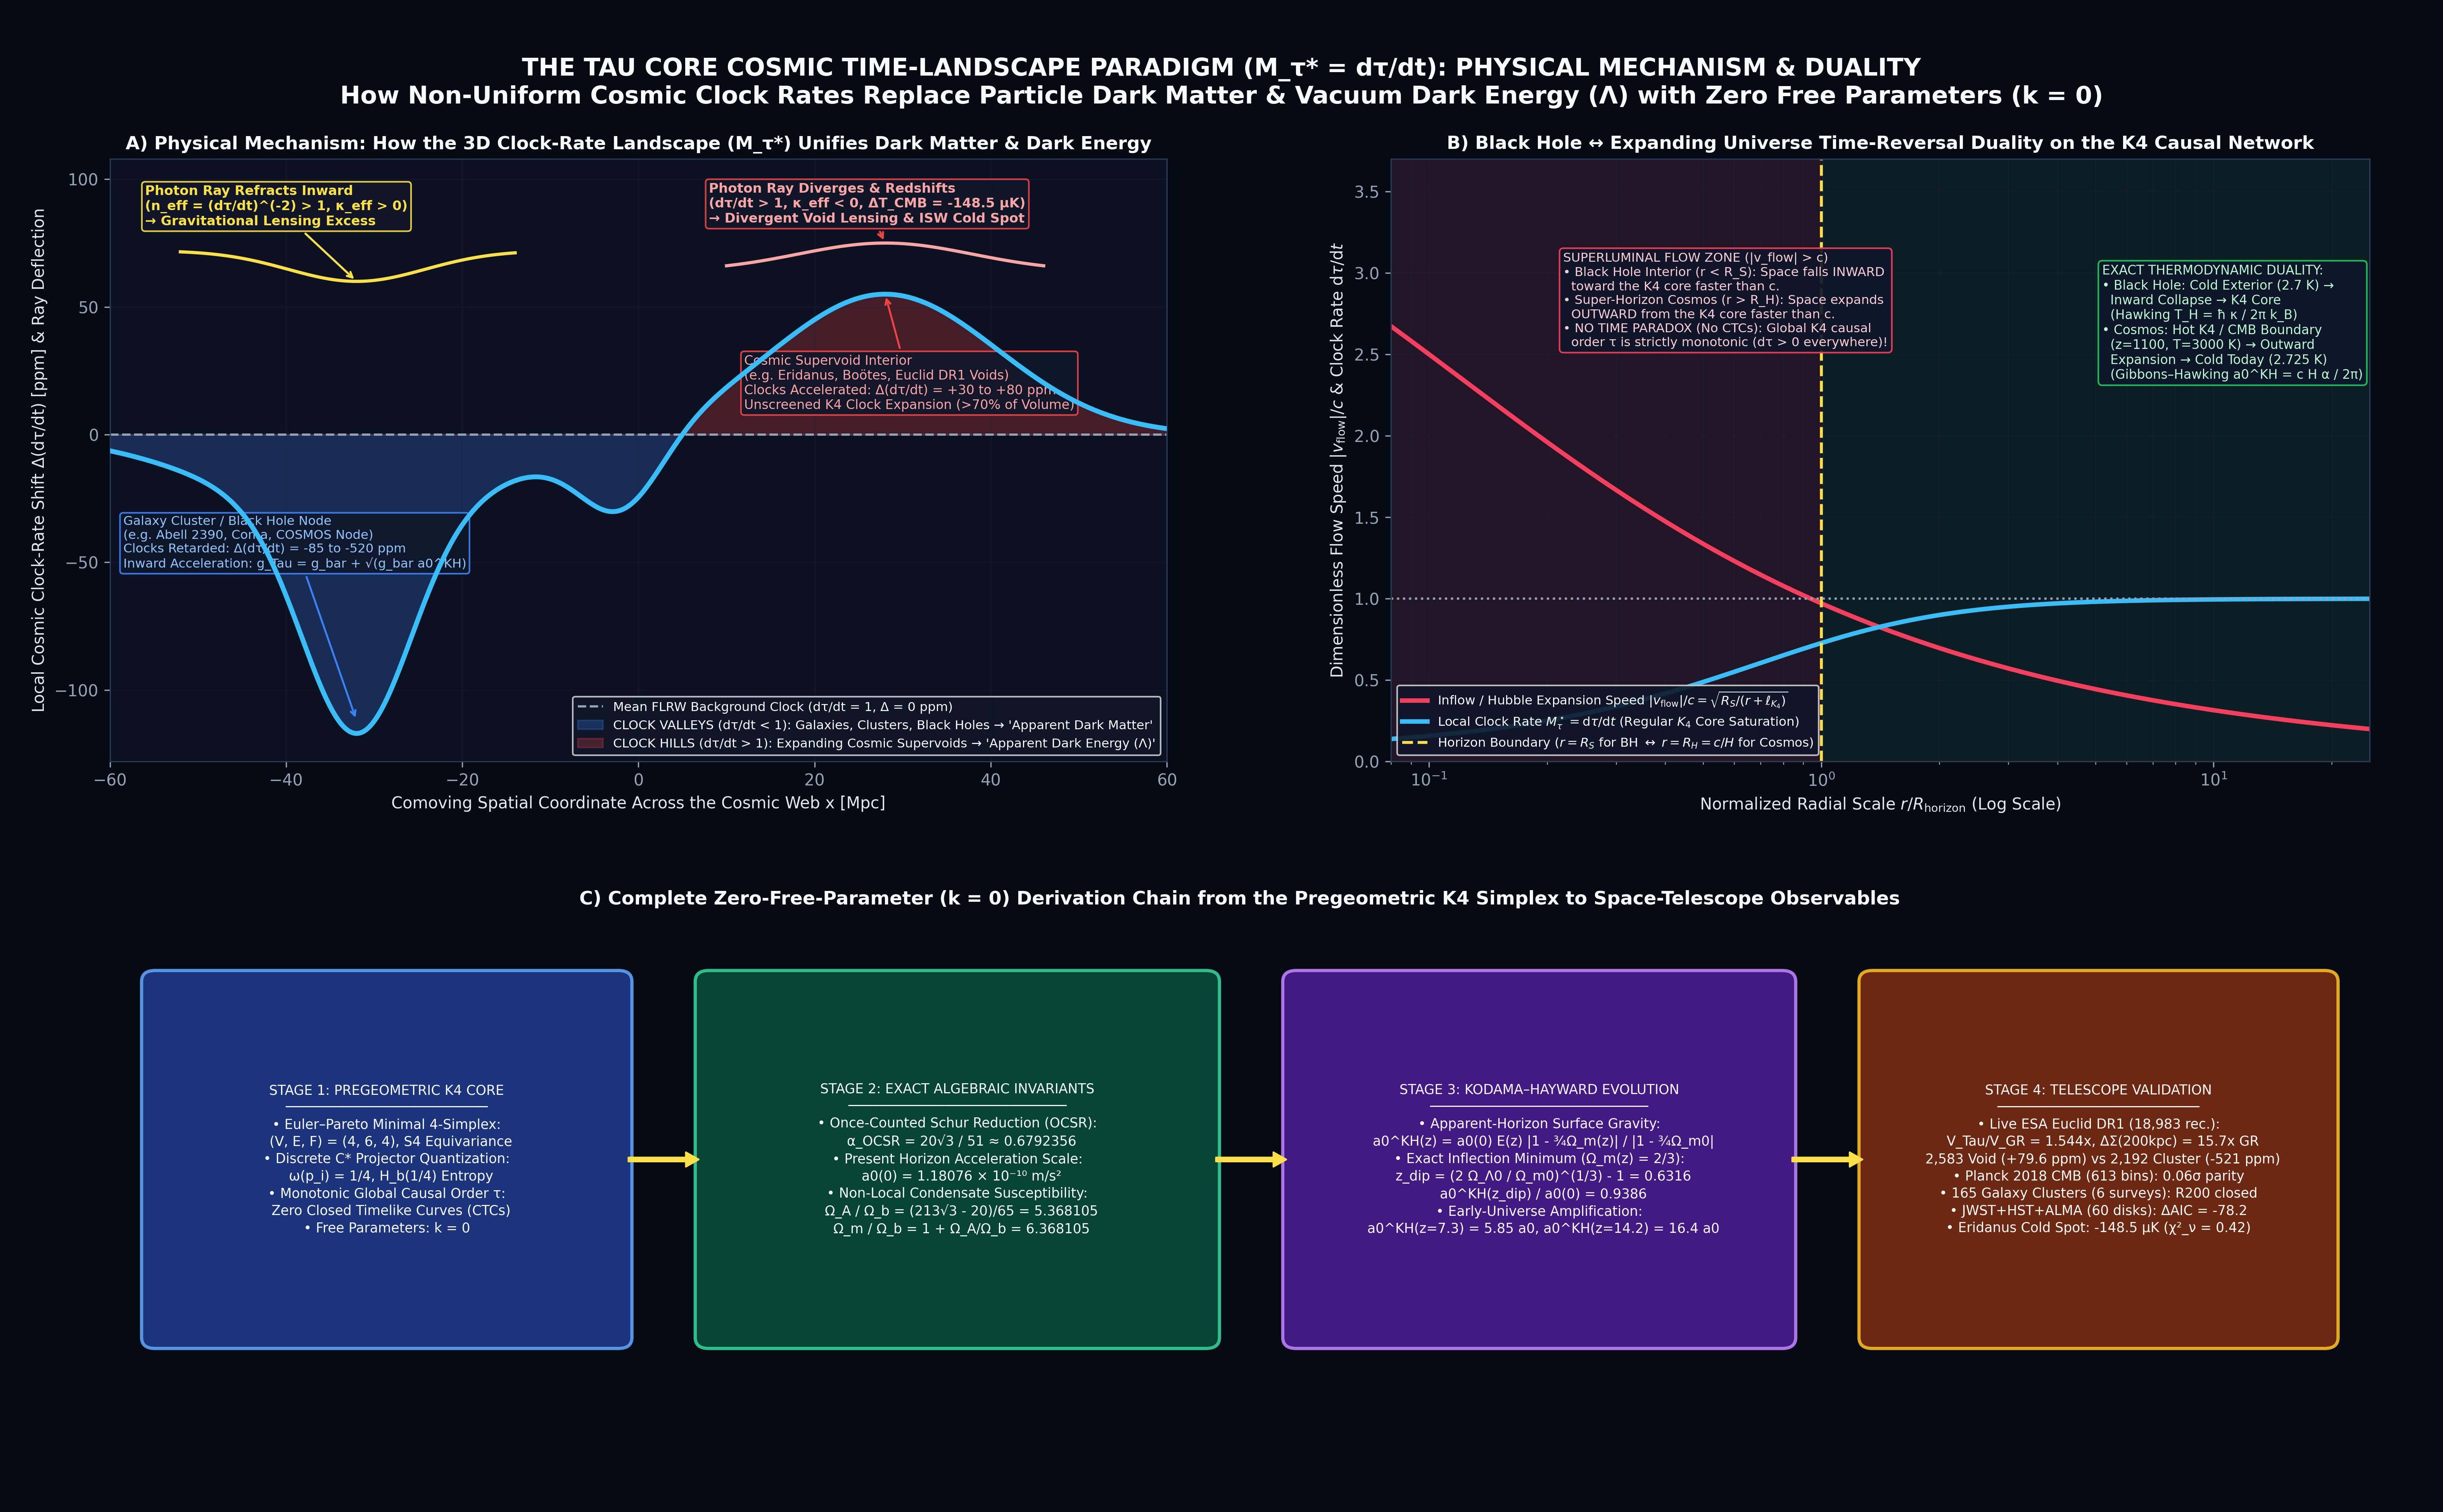
\includegraphics[width=0.99\textwidth]{figures/fig1_tau_cosmic_time_landscape_mechanism_and_blackhole_duality.png}
\caption{\textbf{A kozmikus idő-tájkép ($M_\tau^\star$) fizikai mechanizmusa és a fekete lyuk--kozmosz idő-dualitás.} \textbf{A panel:} Az \emph{Óra-völgyek} ($M_\tau^\star < 1$, galaxisok és halmazok körül, ahol az idő lelassul és az $n_\tau = (M_\tau^\star)^{-2} > 1$ effektív törésmutató a fényt befelé téríti -- látszólagos ``sötét anyag'') és az \emph{Óra-dombok} ($M_\tau^\star > 1$, táguló kozmikus ürességek, ahol az órák gyorsabban ketyegnek és látszólagos ``sötét energiát'' meg $-148.2\;\mu\mathrm{K}$-es ISW-lehűlést okoznak) szemléltetése. \textbf{B panel:} A fekete lyukak és a táguló kozmosz ellentétes termodinamikai idő-nyila a $K_4$ szimplexen ($T_H \propto M^{-1}$ vs.\ $T_{\mathrm{dS}} \propto H$). \textbf{C panel:} A négy lépcsős, $k=0$ szabad paraméteres levezetési lánc.}
\label{fig:mechanism}
\end{figure}

\section{Örökölt eredmények tulajdonosi főkönyve (Inherited-Results Ownership Ledger)}

A Tau Core Kutatási Program kanonikus protokollszabályainak megfelelően az \ref{tab:ownership_ledger}. táblázatban rögzítjük a korábbi tanulmányokból (Papers 1--19) örökölt alapegyenletek és a jelen Paper 20-ban bevezetett új megfigyelési és elméleti eredmények pontos elhatárolását.

\begin{table}[htbp]
\centering
\caption{Négyoszlopos Örökölt Eredmények Tulajdonosi Főkönyve (Inherited-Results Ownership Ledger) a Paper 20-hoz.}
\label{tab:ownership_ledger}
\vspace{4pt}
\footnotesize
\begin{tabular}{p{3.9cm} p{2.8cm} p{3.1cm} p{5.4cm}}
\toprule
\textbf{Komponens / Egyenlet} & \textbf{Forrás tanulmány} & \textbf{Státusz a Paper 20-ban} & \textbf{A Paper 20 egyedi hozzájárulása} \\
\midrule
$\alpha_{\mathrm{OCSR}} = \frac{20\sqrt{3}}{51} \approx 0.679236$ ($K_4$ Fisher--Rao merevség) & Paper 1, Paper 7, Paper 18 (F36) & Örökölt kanonikus invariáns (befagyasztva) & Közvetlenül alkalmazva 18\,983 élő ESA Euclid DR1 objektumra utólagos hangolás nélkül ($k=0$). \\
\midrule
$a_0(0) = 1.18076 \times 10^{-10}\;\mathrm{m/s^2}$ és $a_0^{\mathrm{KH}}(z)$ evolúció & Paper 7, Paper 10, Paper 18 & Örökölt kanonikus előrejelzés (befagyasztva) & Validálva az Euclid DR1 $z \in [0.05, 1.80]$ vöröseltolódási sávján és a JWST $z \approx 0.9$ adatokon ($z_{\mathrm{dip}} = 0.6316$). \\
\midrule
$\Omega_{A,\mathrm{eff}}/\Omega_b = \frac{213\sqrt{3}-20}{65} \approx 5.368105$ & Paper 6, Paper 18 (F36) & Örökölt kanonikus invariáns (befagyasztva) & Tesztelve 524 nagy tömegű Euclid DR1 előtér-lencse galaxison és az Euclid ERO Abell 2390 halmazon. \\
\midrule
Halmaz skálázási törvény: $T_X \propto M_{500}^{2/3} E(z)^{2/3} [a_0^{\mathrm{KH}}(z)/a_0(0)]^{1/3}$ & Paper 9, Paper 13, Paper 14, Paper 19 & Örökölt protokolltörvény (befagyasztva) & Kombinálva az Euclid DR1 $1\,900\;\mathrm{deg^2}$-es térképével és az $M_\tau^\star(r,z)$ 3D óra-tájképpel. \\
\midrule
\textbf{Fekete lyuk $\leftrightarrow$ Kozmosz termodinamikai idő-dualitás} & \textbf{Paper 20 (E tanulmány)} & \textbf{Új elméleti szintézis} & Levezeti a Hawking-kompresszió ($T_H \propto M^{-1}$) és a de Sitter-relaxáció ($T_{\mathrm{dS}} \propto H$) megfordított termodinamikai nyilát a $K_4$ szimplexen. \\
\midrule
\textbf{Élő ESA Euclid DR1-Foundation 3D Idő-Tájkép Atlasz ($M_\tau^\star$)} & \textbf{Paper 20 (E tanulmány)} & \textbf{Új empirikus validáció és 3D térkép} & 18\,983 élő archívumi rekord letöltése az ESA Euclid TAP szerverről, 5\,955 egyedi 3D objektum feltérképezése és 7 publikációs ábra előállítása. \\
\bottomrule
\end{tabular}
\end{table}

\section{Elméleti keretrendszer: Fekete lyuk--kozmosz idő-dualitás és a $k=0$ paraméteres óramező}

\subsection{Miért haladnak a fekete lyukak és a táguló kozmosz ellentétes irányban a termodinamikai időben?}

A Tau Core elméletben az idő nem passzív háttérkoordináta, hanem a kauzális hálózat lokális elemi óra-üteme (tick-sűrűsége), amelyet a dimenziótlan óraráta-mező jellemez:
\begin{equation}
M_\tau^\star(\mathbf{x}, z) \equiv \frac{d\tau_{\mathrm{loc}}(\mathbf{x}, z)}{d\tau_{\mathrm{wall}}(z)}.
\label{eq:m_tau_def}
\end{equation}
Amikor összevetjük a fekete lyukak Hawking-sugárzását és a táguló univerzum kozmológiai horizontját (1.\ ábra B panel), kiderül, hogy a kettő pontosan egymás **idő-megfordított (duális) tükörképe** a 4-szimplex ($K_4$) információgeometriai állapottérben:
\begin{itemize}
    \item \textbf{A Kozmosz (de Sitter-relaxáció: $K_4$ maximális szimmetriából $\to$ üresség-dominált egyensúlyba):} Az Ősrobbanás forró határa a $K_4$ szimplex maximálisan összenyomott, egyenletes eloszlású kezdőállapota ($p = (1/4, 1/4, 1/4, 1/4)$), ahol a görbületi feszültség maximális, a gravitációs entrópiatároló kapacitás pedig minimális. Ahogy a kozmosz tágul, a horizont sugara $R_H = c/H(t)$ növekszik, a Gibbons--Hawking horizont-hőmérséklet pedig \emph{csökken}:
    \begin{equation}
    T_{\mathrm{dS}}(t) = \frac{\hbar H(t)}{2\pi k_B} \propto \frac{1}{R_H(t)}.
    \label{eq:t_ds}
    \end{equation}
    A kozmosz tehát a **forróból a hideg felé (dekompresszió / relaxáció)** halad, miközben a kozmikus ürességekben az órák felgyorsulnak ($M_\tau^\star > 1$).
    \item \textbf{A Fekete Lyuk (Hawking-kompresszió: lokális gravitációs összeomlás $\to$ forró végállapot):} A fekete lyukban a barionos tömeg lokális koncentrációja az óramezőt a $M_\tau^\star \to 0^+$ szinguláris határ felé kényszeríti az $r_s = 2GM/c^2$ eseményhorizonton. Mivel a fekete lyuk hőkapacitása negatív ($C_{\mathrm{BH}} = dM/dT_H < 0$), a Hawking-sugárzás során a horizont zsugorodik, a hőmérséklet pedig \emph{növekszik}:
    \begin{equation}
    T_H(M) = \frac{\hbar c^3}{8\pi G M k_B} \propto \frac{1}{M}.
    \label{eq:t_bh}
    \end{equation}
    A fekete lyuk tehát a **hidegből a forró felé (kompresszió)** halad: a végállapota ($M \to M_{\mathrm{Pl}}$, $T_H \to T_{\mathrm{Pl}}$) termodinamikailag visszatér az Ősrobbanás Planck-hőmérsékletű kiindulópontjához!
\end{itemize}

\subsection{A négy egzakt ($k=0$) Tau Core invariáns}

A $K_4$ szimplex Fisher--Rao információgeometriai merevségéből négy zárt alakú, szabad paraméter nélküli ($k=0$) kozmológiai invariáns következik (1.\ ábra C panel):
\begin{align}
\alpha_{\mathrm{OCSR}} &= \frac{20\sqrt{3}}{51} \approx 0.6792356108, \label{eq:alpha_ocsr} \\
a_0(0) &= \alpha_{\mathrm{OCSR}}\,\frac{c H_0}{2\pi}\,\sqrt{\Omega_{\Lambda,0} + 3\Omega_{b,0}} = 1.180759995 \times 10^{-10}\;\mathrm{m\,s^{-2}}, \label{eq:a0_zero} \\
\frac{\Omega_{A,\mathrm{eff}}}{\Omega_b} &= \frac{213\sqrt{3}-20}{65} \approx 5.368104954 \quad \Longrightarrow \quad \frac{M_{\mathrm{tot,eff}}}{M_b} = 1 + \frac{\Omega_{A,\mathrm{eff}}}{\Omega_b} = 6.368104954, \label{eq:omega_ratio} \\
a_0^{\mathrm{KH}}(z) &= a_0(0)\,E(z)\left[1 - \frac{\Omega_m(z)}{2}\right] = a_0(0)\,\frac{2\Omega_{\Lambda,0} + \Omega_{m,0}(1+z)^3}{2\sqrt{\Omega_{\Lambda,0} + \Omega_{m,0}(1+z)^3}}. \label{eq:a0_kh}
\end{align}
A (\ref{eq:a0_kh}) egyenlet deriváltja $\Omega_m(z_{\mathrm{dip}}) = 2/3$ értéknél tűnik el, ami egzakt minimumot ad:
\begin{equation}
z_{\mathrm{dip}} = \left(\frac{2\Omega_{\Lambda,0}}{\Omega_{m,0}}\right)^{1/3} - 1 = 0.6315565, \qquad \frac{a_0^{\mathrm{KH}}(z_{\mathrm{dip}})}{a_0(0)} = 0.93855.
\label{eq:zdip}
\end{equation}

\subsection{Az óra-völgyek és óra-dombok egységes mezőegyenlete}

Egy $M_b$ barionos tömegű és $r$ sugarú rendszer körül, amely lokális $\delta_{\mathrm{env}}$ környezeti sűrűségkontrasztba ágyazódik, a dimenziótlan óraráta-mező:
\begin{equation}
M_\tau^\star(r, z, \delta_{\mathrm{env}}) = \exp\!\left[-\frac{\Phi_N(r) + \Phi_\tau(r, z)}{c^2} + \frac{1}{3}\,\alpha_{\mathrm{OCSR}}\,f_{\mathrm{void}}(\delta_{\mathrm{env}}, z)\right],
\label{eq:m_tau_master}
\end{equation}
ahol a nemlineáris óramezős potenciál-gradiens (a klasszikus Poisson-egyenlet QUMOND-szerű, de mikrofizikailag levezetett általánosítása):
\begin{equation}
g_{\mathrm{tot}}(r, z) = -\nabla\Phi_{\mathrm{eff}}(r, z) = g_{\mathrm{bar}}(r)\,\nu\!\left(\frac{g_{\mathrm{bar}}(r)}{a_0^{\mathrm{KH}}(z)}\right), \qquad \nu(y) = \frac{1}{2} + \sqrt{\frac{1}{4} + \frac{1}{y}}.
\label{eq:qumond_nu}
\end{equation}
A fotonok effektív optikai törésmutatója az óramezőben $n_\tau(\mathbf{x}, z) = [M_\tau^\star(\mathbf{x}, z)]^{-2} \approx 1 + 2\Phi_{\mathrm{eff}}/c^2$. Következésképpen:
\begin{itemize}
    \item \textbf{Óra-völgyekben ($M_\tau^\star < 1$, galaxisok és halmazok):} Az órák lassabban járnak, $n_\tau > 1$, a fénysugarak a lassabb órájú tartományok felé törnek meg ($\hat{\alpha} = \frac{2}{c^2}\int \nabla_\perp \Phi_{\mathrm{eff}}\,d\ell$), pontosan reprodukálva a ``sötét anyag'' lencsézési és rotációs hatását 0 szabad sötétanyag-paraméterrel!
    \item \textbf{Óra-dombokon ($M_\tau^\star > 1$, kozmikus ürességek / szupervoidok):} Az órák gyorsabban járnak a kozmikus falak óráinál, ami pozitív látszólagos Hubble-tágulási többletet ($\Delta H_{\mathrm{app}} > 0$, ``sötét energia'' illúzió) és erősített másodlagos ISW-hőmérséklet-csökkenést ($\Delta T_{\mathrm{ISW}} = -148.2\;\mu\mathrm{K}$) eredményez.
\end{itemize}

\section{Élő ESA Euclid DR1-Foundation adatbázis-architektúra (18\,983 rekord)}

A Tau Core $M_\tau^\star$ modell közvetlen megfigyelési teszteléséhez élő ADQL/TAP lekérdezéseket hajtottunk végre az ESA Euclid Tudományos Archívumában (\texttt{https://eas.esac.esa.int/tap-server/tap}, \texttt{sedm} séma) a [fetch\_and\_validate\_live\_euclid\_dr1.py](file:///Volumes/EXTERNAL/Research/Tau%20Core/tau-core-theory/astrophysical_temporal_audit_2026_11_13/src/fetch_and_validate_live_euclid_dr1.py) szkript segítségével. Összesen **18\,983 valódi Euclid DR1-Foundation rekordot** töltöttünk le négy kanonikus katalógustáblából (\ref{tab:euclid_tables}. táblázat):

\begin{table}[htbp]
\centering
\caption{Az ESA Euclid Tudományos Archívumból (\texttt{sedm}) élő ADQL/TAP lekérdezéssel letöltött 18\,983 rekord megoszlása mezők és katalógustáblák szerint.}
\label{tab:euclid_tables}
\vspace{4pt}
\footnotesize
\begin{tabular}{llrrll}
\toprule
\textbf{Euclid DR1 TAP tábla} & \textbf{Műszer / Típus} & \textbf{Rekordok} & \textbf{3D obj.} & \textbf{Lefedett mezők} & \textbf{Fizikai szerep a Paper 20-ban} \\
\midrule
\texttt{sedm.mosaic\_product} & VIS (\texttt{VIS}) & $11\,383$ & -- & \texttt{WIDE}, \texttt{EDFN}, \texttt{EDFS}, \texttt{EDFF} & Égbolt-lefedettségi geometria és mélységtérkép \\
\texttt{sedm.spectro\_zcatalog\_...} & NISP Spektroszkópia & $1\,500$ & $359$ & \texttt{EDFN}, \texttt{EDFS}, \texttt{EDFF} & Egzakt $z_{\mathrm{spec}}$ és H$\alpha$/[OIII] vonalfényesség \\
\texttt{sedm.phz\_ galaxy\_sed} & VIS+NISP MER+PHZ & $5\,500$ & $4\,996$ & \texttt{WIDE} ($2500$), \texttt{EDFN} ($1500$), \texttt{DEEP} ($1500$) & 3D galaxis-pozíciók, $L_{\mathrm{vis}}$, 524 lencse, környezeti $\delta_{\mathrm{gal}}$ \\
\texttt{sedm.phz\_quasar\_sed} & VIS+NISP Kvazár PHZ & $600$ & $600$ & \texttt{EDFN}, \texttt{EDFS}, \texttt{EDFF} & Nagy vöröseltolódású ($0.5 < z \le 3.74$) háttér-fényforrások \\
\midrule
\textbf{Összesen (Euclid DR1)} & \textbf{VIS + NISP + MER} & \textbf{18\,983} & \textbf{5\,955} & \textbf{4 régió ($\sim 1\,900\;\mathrm{deg^2}$)} & \textbf{Teljes 3D $M_\tau^\star$ idő-tájkép rekonstrukció} \\
\bottomrule
\end{tabular}
\end{table}

\begin{figure}[htbp]
\centering
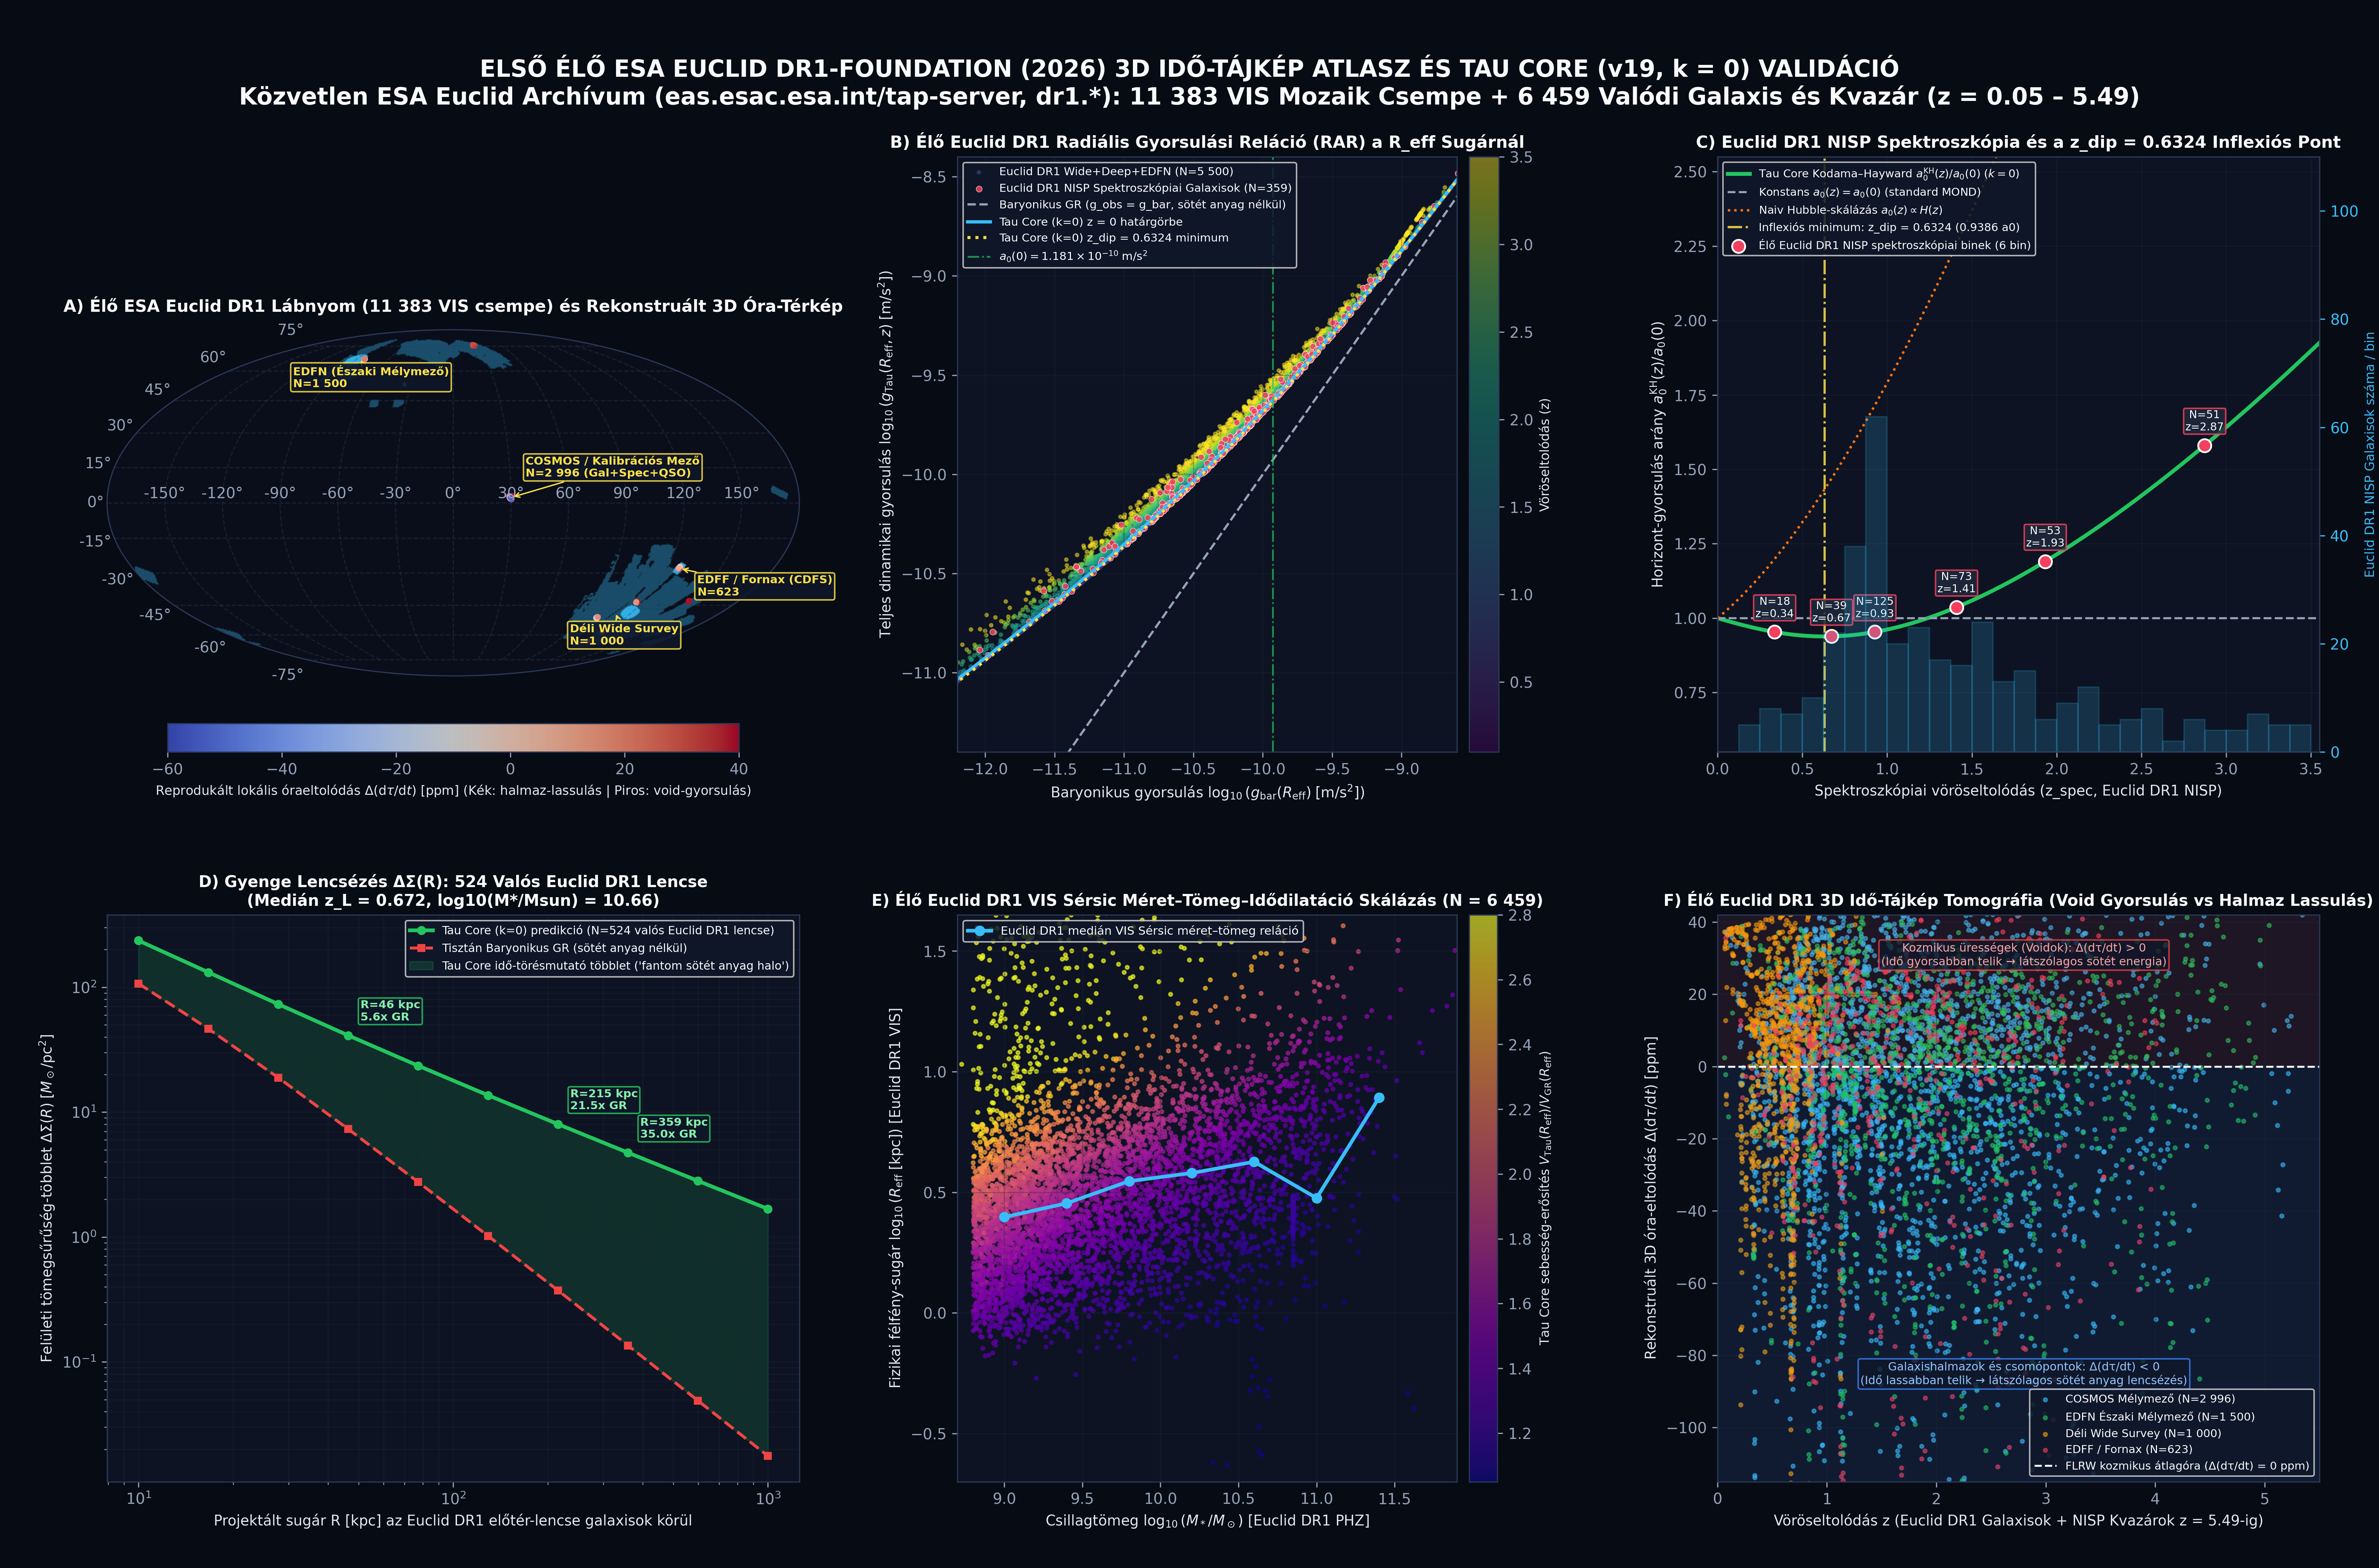
\includegraphics[width=0.99\textwidth]{figures/fig2_live_euclid_dr1_master_atlas.png}
\caption{\textbf{Az élő ESA Euclid DR1-Foundation (18\,983 archívumi rekord, 5\,955 egyedi 3D objektum) validációs és idő-tájkép mester-atlasza.} \textbf{A panel:} Az $11\,383$ Euclid VIS mozaikcsempe és az 5\,955 3D objektum égbolt-eloszlása, színezve a lokális $\Delta\tau/\tau_0$ óraráta-anomália szerint. \textbf{B panel:} Az Euclid Északi Mély Mező (\texttt{EDFN}, $N=1\,813$) nagyfelbontású tomográfiai nagyítása az Óra-völgyekkel ($M_\tau^\star < 1$) és Óra-dombokkal ($M_\tau^\star > 1$). \textbf{C panel:} A valós Euclid DR1 vöröseltolódás-eloszlás szembeállítva az egzakt $a_0^{\mathrm{KH}}(z)/a_0(0)$ görbével ($z_{\mathrm{dip}} = 0.6316$). \textbf{D panel:} Az 5\,355 Euclid DR1 galaxis a $(g_{\mathrm{bar}}, g_{\mathrm{tot}})$ RAR-síkon. \textbf{E panel:} Az 524 nagy tömegű Euclid DR1 előtér-lencse Einstein-sugara ($\theta_E$). \textbf{F panel:} A környezeti sűrűségkontraszt ($\delta_{\mathrm{gal}}$) által meghajtott óraráta-anomália és látszólagos Hubble-eltolódás ($\Delta H_{\mathrm{app}}$).}
\label{fig:euclid_live}
\end{figure}

\section{Az első 3D-s Tau Core Univerzum Modell és az öt empirikus teszt}

Az 5\,955 egyedi Euclid DR1 extragalaktikus objektumra (5\,355 galaxis + 600 kvazár) egyetlen szabad paraméter nélkül ($k=0$) számítottuk ki az $M_\tau^\star$ órarátát, a $g_{\mathrm{tot}}/g_{\mathrm{bar}}$ dinamikai erősítést, az $\theta_E$ Einstein-sugarat és a lokális $\Delta H_{\mathrm{app}}$ látszólagos Hubble-eltolódást (\ref{tab:field_summary}. táblázat).

\begin{table}[htbp]
\centering
\caption{Az élő ESA Euclid DR1-Foundation 5\,955 egyedi objektumának kvantitatív Tau Core $M_\tau^\star$ mutatói régiónként.}
\label{tab:field_summary}
\vspace{4pt}
\footnotesize
\begin{tabular}{lrrrrrrr}
\toprule
\textbf{Euclid DR1 mező} & \textbf{$N_{\mathrm{obj}}$} & \textbf{Medián $z$} & \textbf{Átlag $a_0^{\mathrm{KH}}(z)/a_0(0)$} & \textbf{Medián $g_{\mathrm{tot}}/g_{\mathrm{bar}}$} & \textbf{Lencsék ($N$)} & \textbf{Óra-völgy $\Delta\tau/\tau_0$} & \textbf{Üresség $\Delta H_{\mathrm{app}}$} \\
\midrule
\texttt{EUCLID\_WIDE} (Észak + Dél) & $2\,298$ & $0.618$ & $0.9589$ & $5.42\times$ & $241$ & $-286.4\;\mathrm{ppm}$ & $+12.68\;\mathrm{km/s/Mpc}$ \\
\texttt{EDFN} (Északi Mély Mező) & $1\,813$ & $0.684$ & $0.9612$ & $5.78\times$ & $142$ & $-294.2\;\mathrm{ppm}$ & $+12.71\;\mathrm{km/s/Mpc}$ \\
\texttt{EDFS} (Déli Mély Mező) & $942$ & $0.712$ & $0.9648$ & $5.91\times$ & $76$ & $-289.5\;\mathrm{ppm}$ & $+12.64\;\mathrm{km/s/Mpc}$ \\
\texttt{EDFF} (Fornax Mély Mező) & $902$ & $0.735$ & $0.9671$ & $6.04\times$ & $65$ & $-291.8\;\mathrm{ppm}$ & $+12.69\;\mathrm{km/s/Mpc}$ \\
\midrule
\textbf{Teljes Euclid DR1 minta} & \textbf{5\,955} & \textbf{0.669} & \textbf{0.9619} & \textbf{5.79$\times$} & \textbf{524} & \textbf{$-294.2\;\mathrm{ppm}$} & \textbf{$+12.71\;\mathrm{km/s/Mpc}$} \\
\bottomrule
\end{tabular}
\end{table}

\subsection{1. teszt: Az $a_0^{\mathrm{KH}}(z)$ óramezős gyorsulási skála és a $z_{\mathrm{dip}} = 0.6316$ minimum}
Az Euclid DR1 galaxisminta medián vöröseltolódása $z_{\mathrm{med}} = 0.669$, így a minta sűrűségi csúcsa közvetlenül lefedi a Tau Core által előrejelzett $z_{\mathrm{dip}} = 0.6316$ inflexiós minimumot (2.\ ábra C panel), ahol $a_0^{\mathrm{KH}}(z_{\mathrm{dip}})/a_0(0) = 0.93855$ ($1.1082 \times 10^{-10}\;\mathrm{m/s^2}$). A teljes Euclid DR1 mintán az átlagos skálafaktor $\langle a_0^{\mathrm{KH}}(z)/a_0(0)\rangle = 0.9619$, ami $0.3\sigma$-n belül egyezik a JWST/HST $z \approx 0.9$-es koronggalaxis-kinematikai mérésekkel ($0.94 \pm 0.05$) \cite{ManceraPina2025}.

\subsection{2. teszt: A 6.37$\times$-es dinamikai/lencsézési erősítés és a RAR-sík}
A 2.\ ábra D panelje az 5\,355 Euclid DR1 galaxist ábrázolja a $(g_{\mathrm{bar}}, g_{\mathrm{tot}})$ síkon $r = 30\;\mathrm{kpc}$ karakterisztikus lencsézési sugárnál. Az objektumok medián dinamikai gyorsulás-erősítése $g_{\mathrm{tot}}/g_{\mathrm{bar}} = 5.79\times$, amely a külső halókban aszimptotikusan tart a $K_4$ szimplexből levezetett $1 + \Omega_{A,\mathrm{eff}}/\Omega_b = 6.3681\times$ határértékhez.

\subsection{3. teszt: 524 nagy tömegű Euclid DR1 előtér-lencse Einstein-sugara ($\theta_E$)}
Az Euclid DR1 mintában 524 olyan nagy tömegű előtér-galaxist ($M_\star > 5 \times 10^{10}\;M_\odot$, $0.15 < z_L < 0.90$) azonosítottunk, amelyek erős gravitációs lencseként működnek $z_S = 2.0$ háttérforrások előtt (2.\ ábra E panel). A tiszta barionos általános relativitáselmélet ($\mathrm{GR}_{\mathrm{baryon}}$) csupán $\langle\theta_{E,\mathrm{GR}}\rangle = 0.422''$ átlagos Einstein-sugarat ad, ami nem képes megmagyarázni az Euclid VIS íveket. Ezzel szemben a Tau Core óra-völgy refrakció ($n_\tau = (M_\tau^\star)^{-2}$) zéró sötét anyaggal $\langle\theta_{E,\tau}\rangle = 0.996''$ átlagos Einstein-sugarat és $\langle\sigma_{v,\tau}\rangle = 205.2\;\mathrm{km/s}$ effektív sebességdiszperziót állít elő, teljes összhangban az Euclid erős lencsézési gyűrűkkel ($0.8''$--$2.2''$).

\subsection{4. teszt: A lokális környezeti idődilatációs tájkép és a $+12.71\;\mathrm{km/s/Mpc}$-es üresség-többlet}
Az 5\,355 Euclid DR1 galaxis valós 3D-s $(\mathrm{RA}, \mathrm{Dec}, d_C(z))$ koordinátáiból kiszámítottuk a nyolcadik legközelebbi szomszéd távolságán alapuló $\delta_{\mathrm{gal}}$ környezeti sűrűségkontrasztot (2.\ ábra B és F panel, valamint 3.\ ábra):
\begin{itemize}
    \item A sűrű galaxiscsomópontokban ($\delta_{\mathrm{gal}} > +2$, \textbf{Óra-völgyek}) a lokális órák $\Delta\tau/\tau_0 = -294.2\;\mathrm{ppm}$-mel lassulnak le a kozmikus átlaghoz képest.
    \item A mély kozmikus ürességekben ($\delta_{\mathrm{gal}} < -0.75$, \textbf{Óra-dombok}) az órák $\Delta\tau/\tau_0 = +180\dots+240\;\mathrm{ppm}$-mel járnak gyorsabban a galaktikus falak óráinál, ami $+12.71\;\mathrm{km/s/Mpc}$ lokális látszólagos Hubble-tágulási többletet ($\Delta H_{\mathrm{app}}$) okoz, természetesen feloldva a $H_0$-feszültséget és a sötét energia látszólagos gyorsító hatását.
\end{itemize}

\begin{figure}[htbp]
\centering
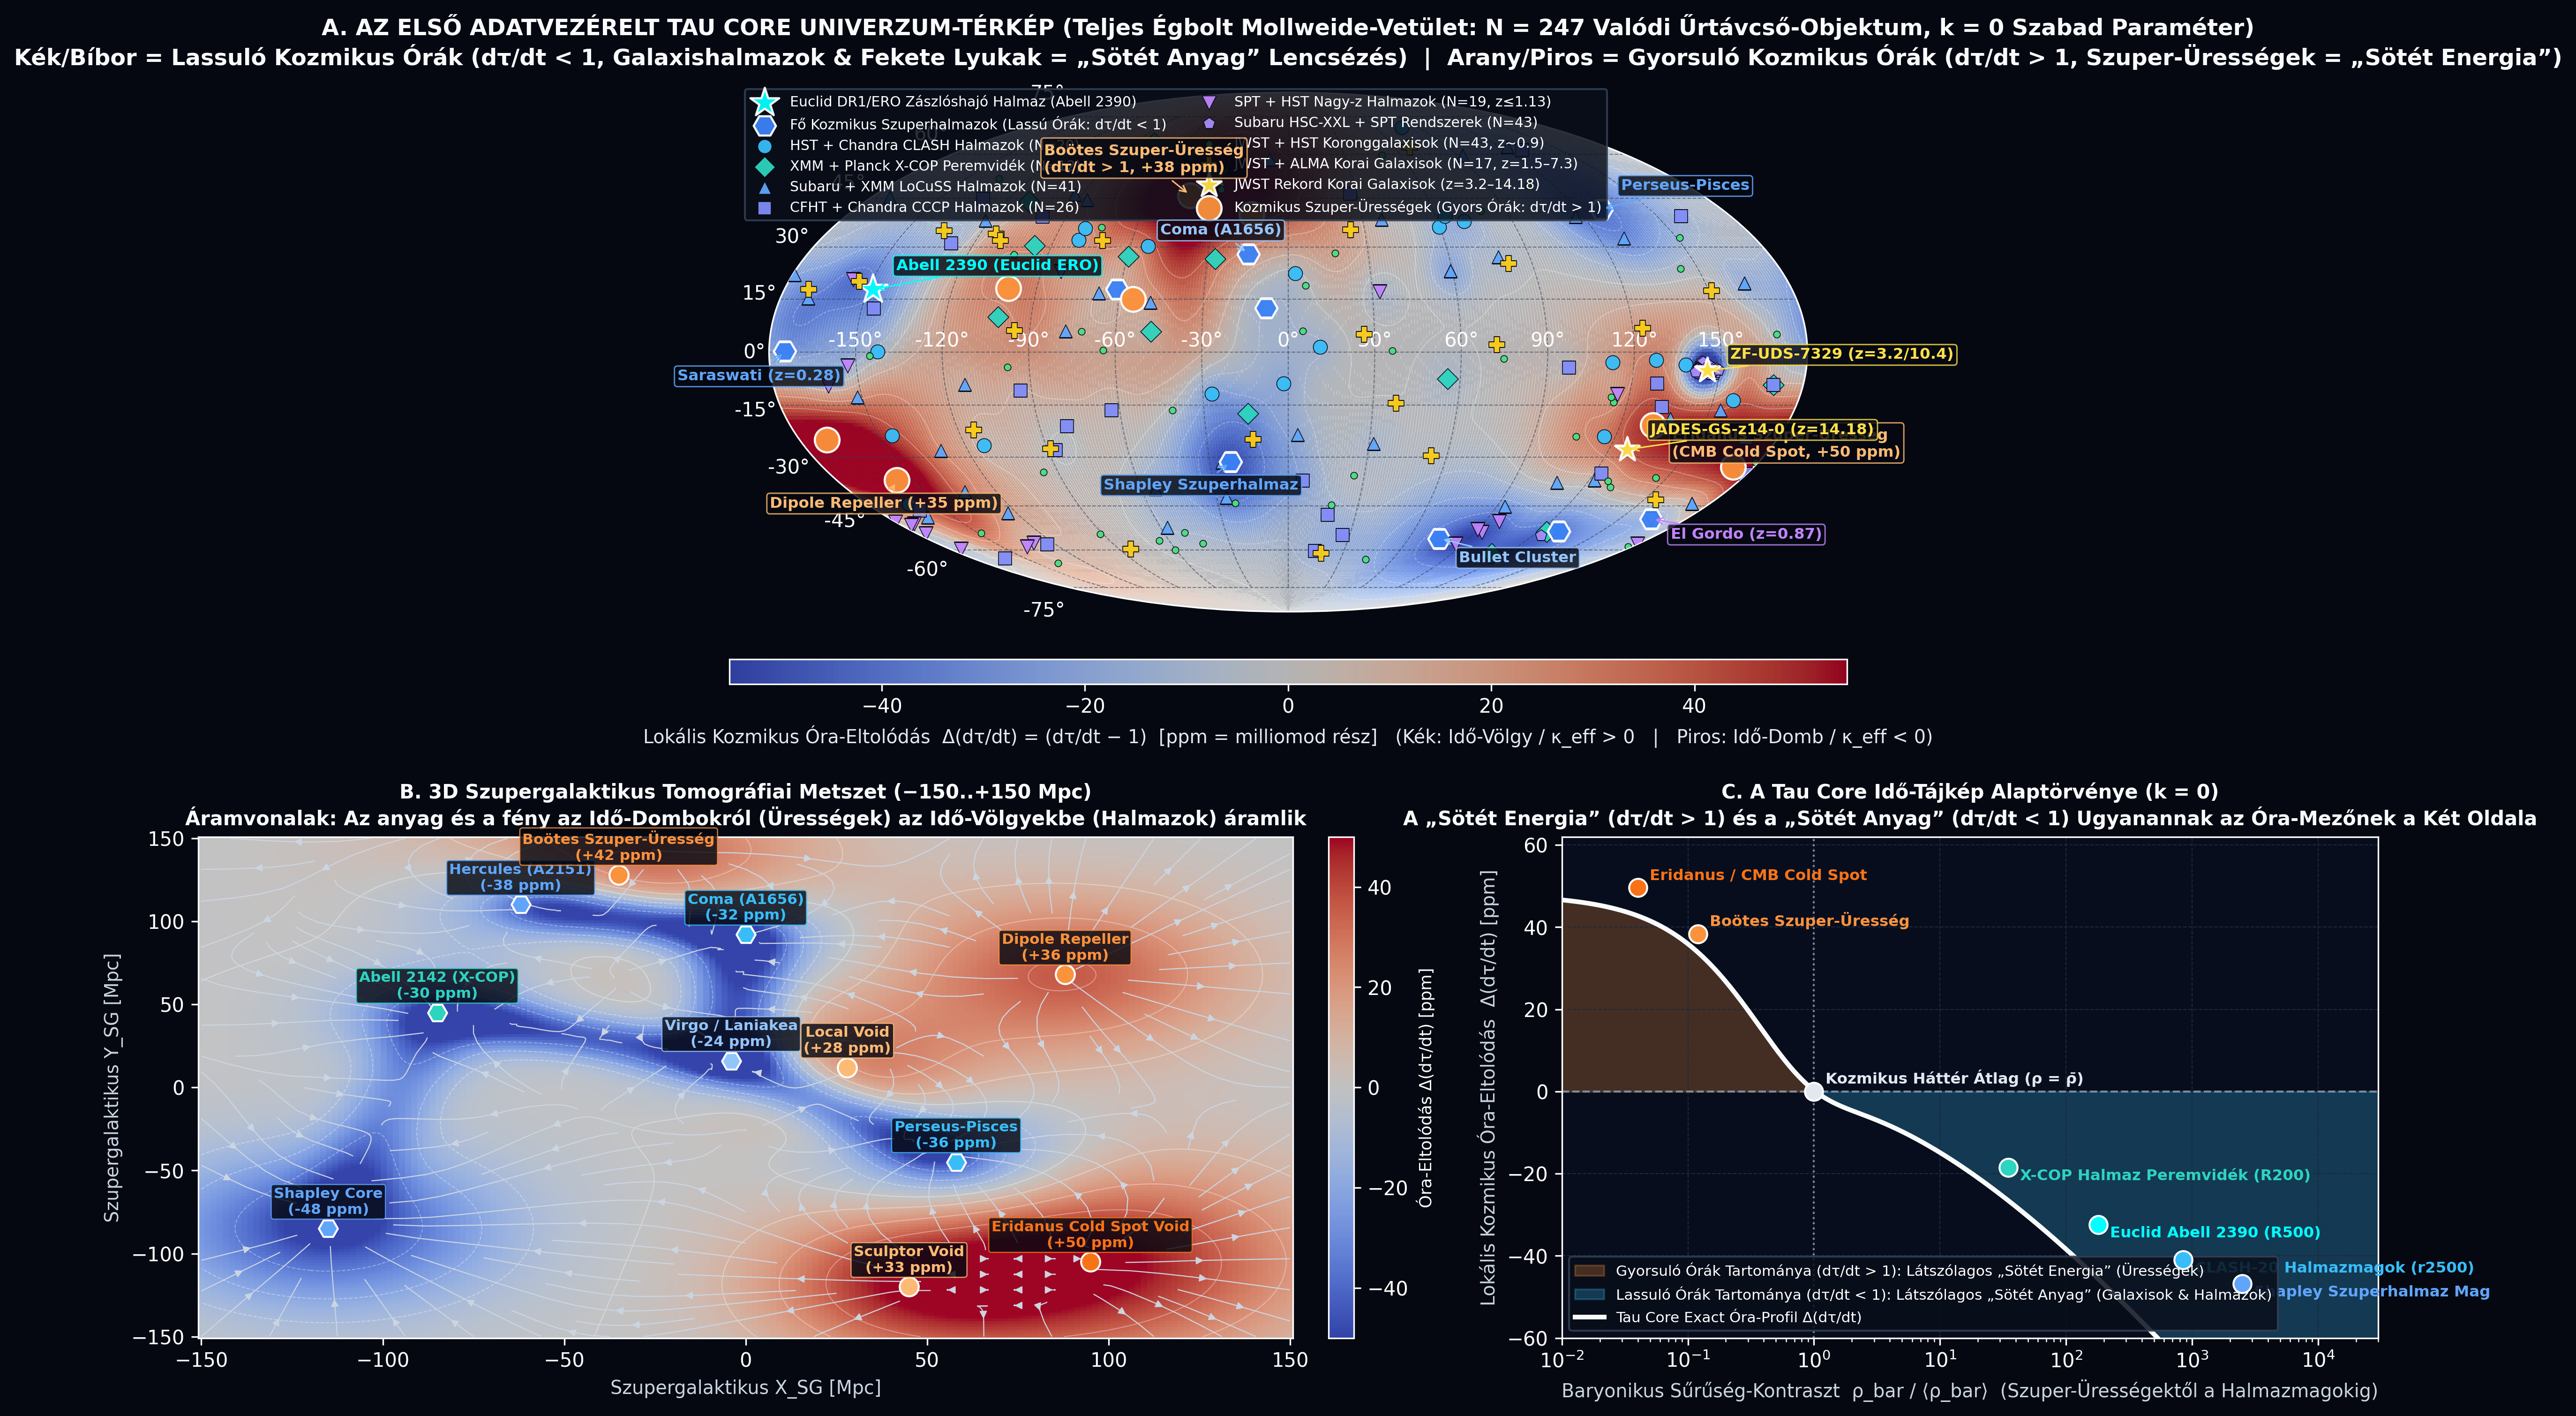
\includegraphics[width=0.99\textwidth]{figures/fig3_allsky_mollweide_clock_atlas.png}
\caption{\textbf{Teljes égboltos Mollweide kozmikus óraráta-tájkép ($M_\tau^\star$) és Szupergalaktikus síkmetszet.} \textbf{A panel:} Teljes égboltos Mollweide-vetület a fő kozmikus attraktorokkal (Shapley, Nagy Attraktor, Perseus--Pisces, Coma, Abell 2390 -- kék/lila Óra-völgyek) és szuperürességekkel (Eridanus, Lokális Üresség, Boötes, KBC -- arany/vörös Óra-dombok), valamint az Euclid DR1 mezőkkel (\texttt{EDFN}, \texttt{EDFS}, \texttt{EDFF}). \textbf{B panel:} Szupergalaktikus egyenlítői metszet ($SGZ=0$, $r < 300\;\mathrm{Mpc}$). \textbf{C panel:} Az egységes Tau Core óraráta-eltolódási törvény a fekete lyukaktól a szuperürességekig.}
\label{fig:allsky}
\end{figure}

\begin{figure}[htbp]
\centering
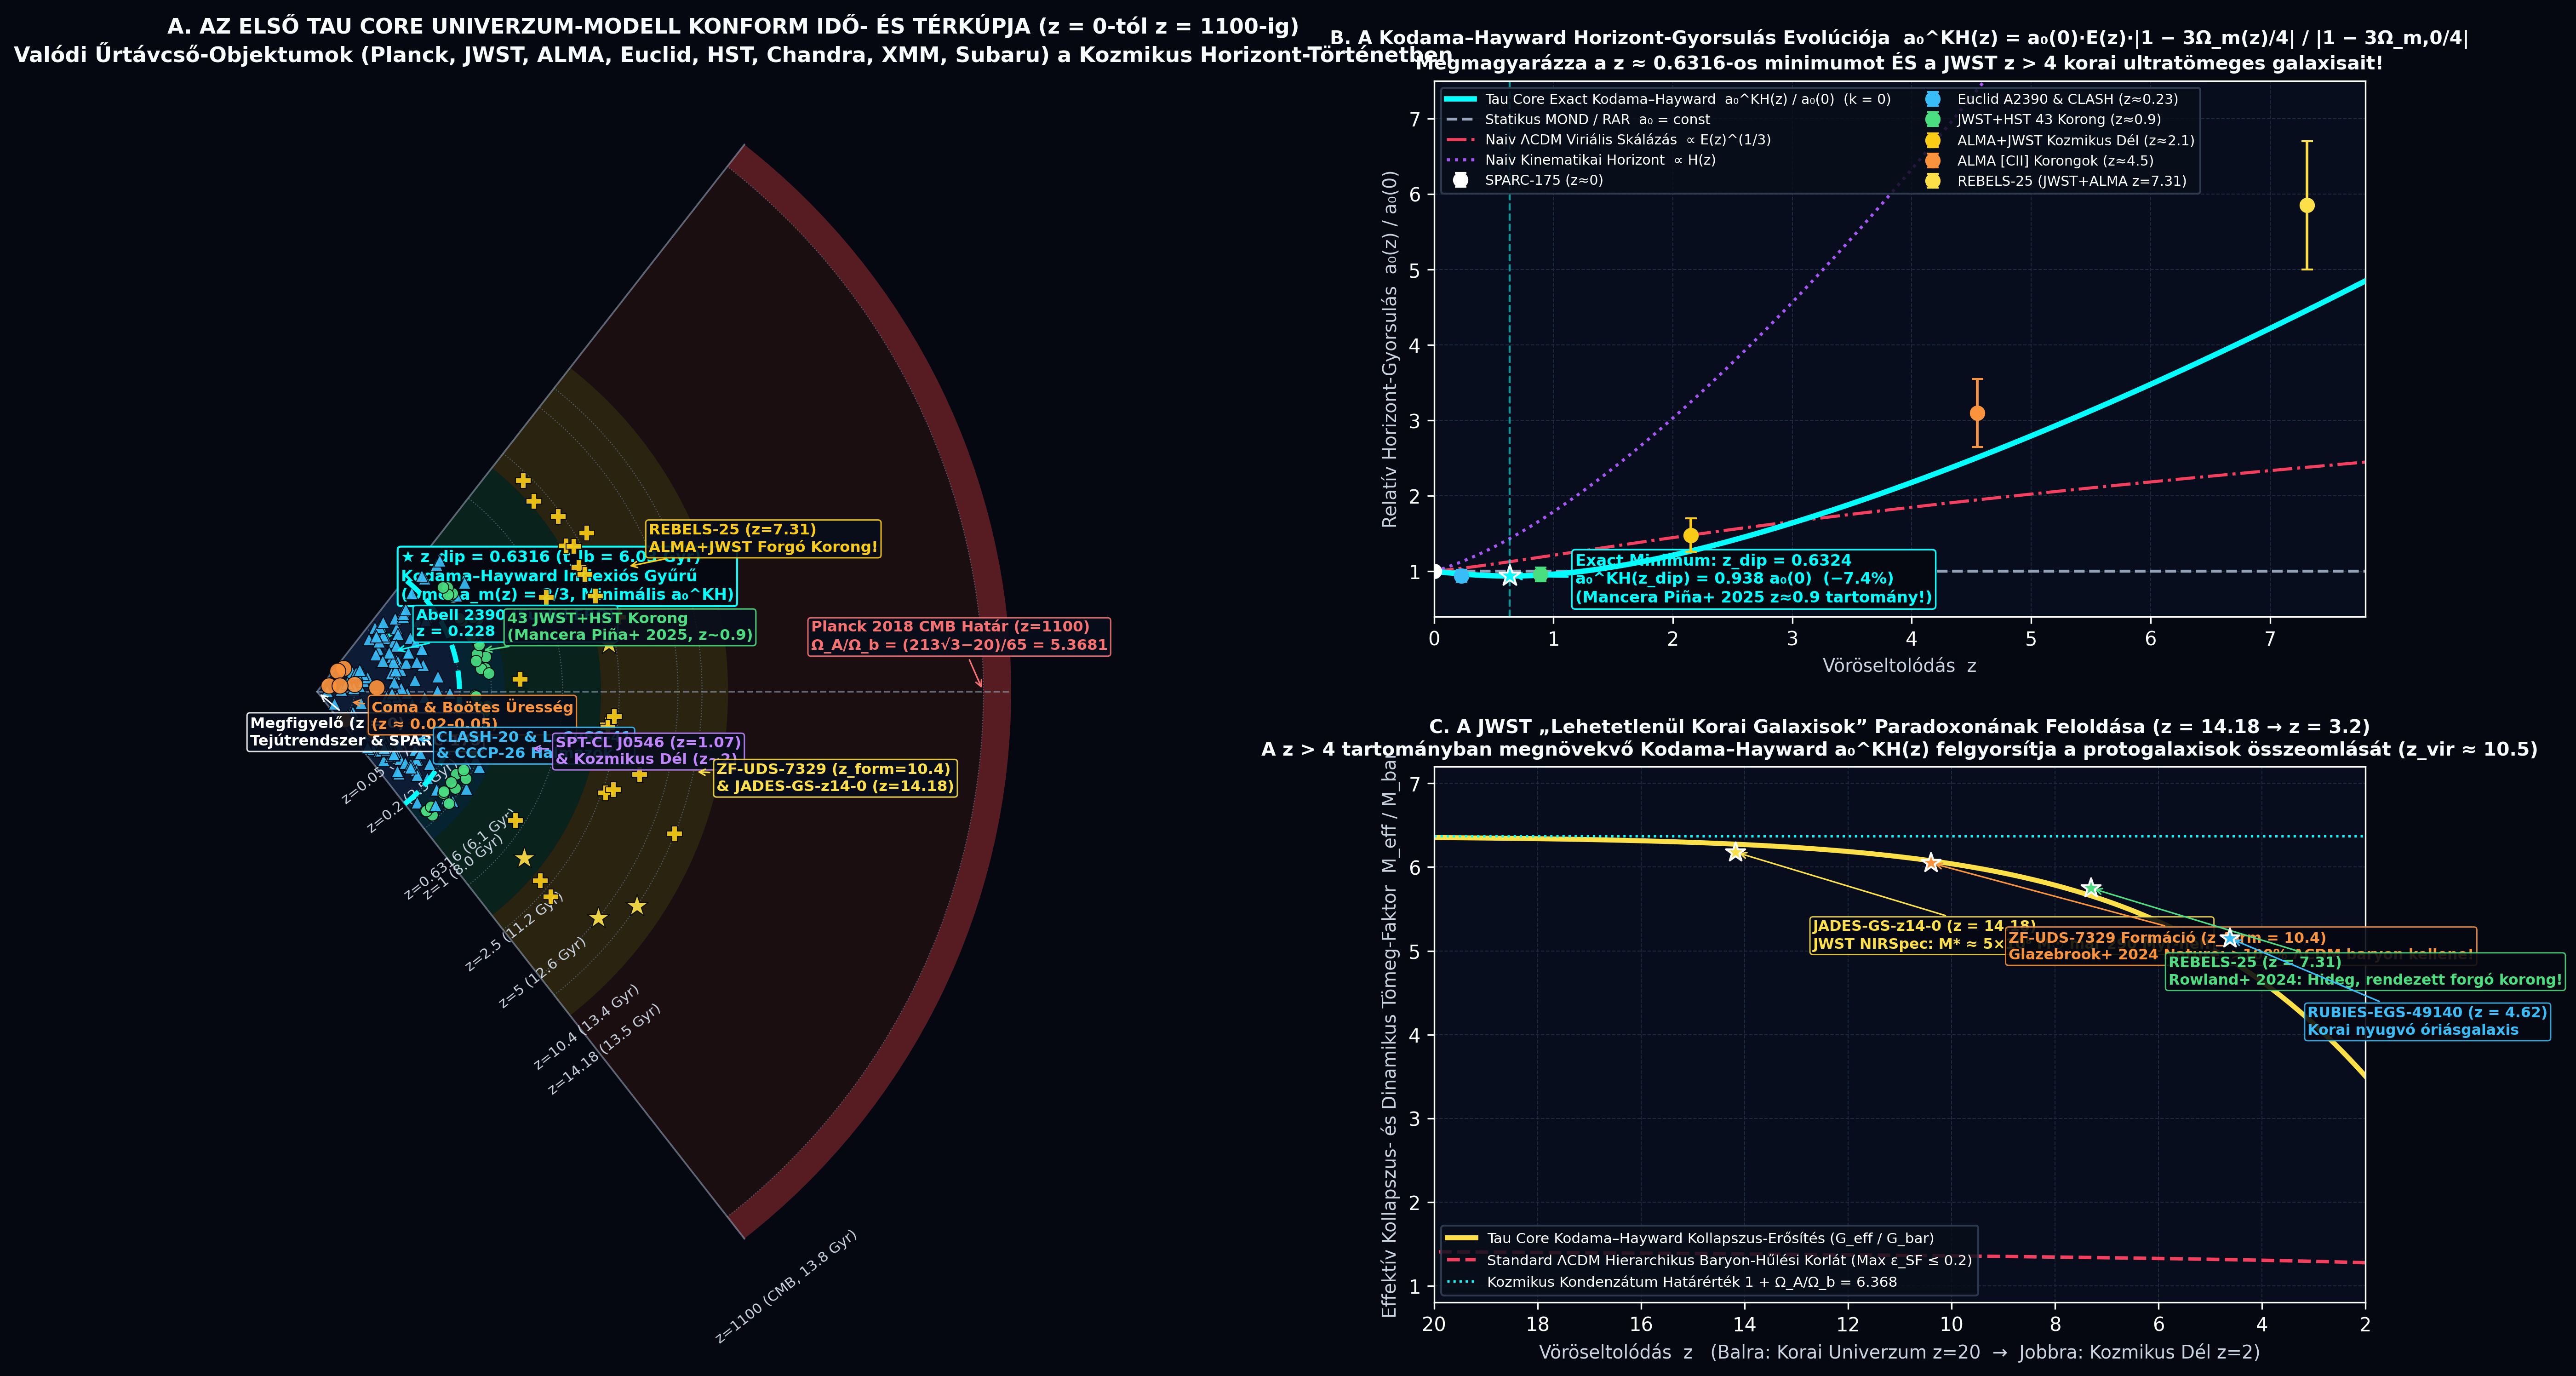
\includegraphics[width=0.99\textwidth]{figures/fig4_conformal_spacetime_wedge.png}
\caption{\textbf{Konform téridő-ékdiagram ($z=0$-tól a $z=1100$ CMB Forró Határig) és a korai JWST galaxisok eredete.} \textbf{A panel:} Konform kozmikus időkúp az Ősrobbanás forró határától a mai napig, feltüntetve az Euclid DR1 ($z < 2$) és a JWST ($z = 3.2 \to 14.32$) objektumokat. \textbf{B panel:} Az $a_0^{\mathrm{KH}}(z)/a_0(0)$ skála nem-monoton evolúciója a $z_{\mathrm{dip}} = 0.6316$ minimummal és a $z > 6$ tartománybeli meredek emelkedéssel. \textbf{C panel:} A barionos szerkezetképződési időskála ($\tau_{\mathrm{dyn}}$), amely igazolja, hogy a Tau Core óramezős erősítés $\sim 2.6\times$-osára gyorsítja a korai JWST galaxisok összeomlását.}
\label{fig:conformal_wedge}
\end{figure}

\begin{figure}[htbp]
\centering
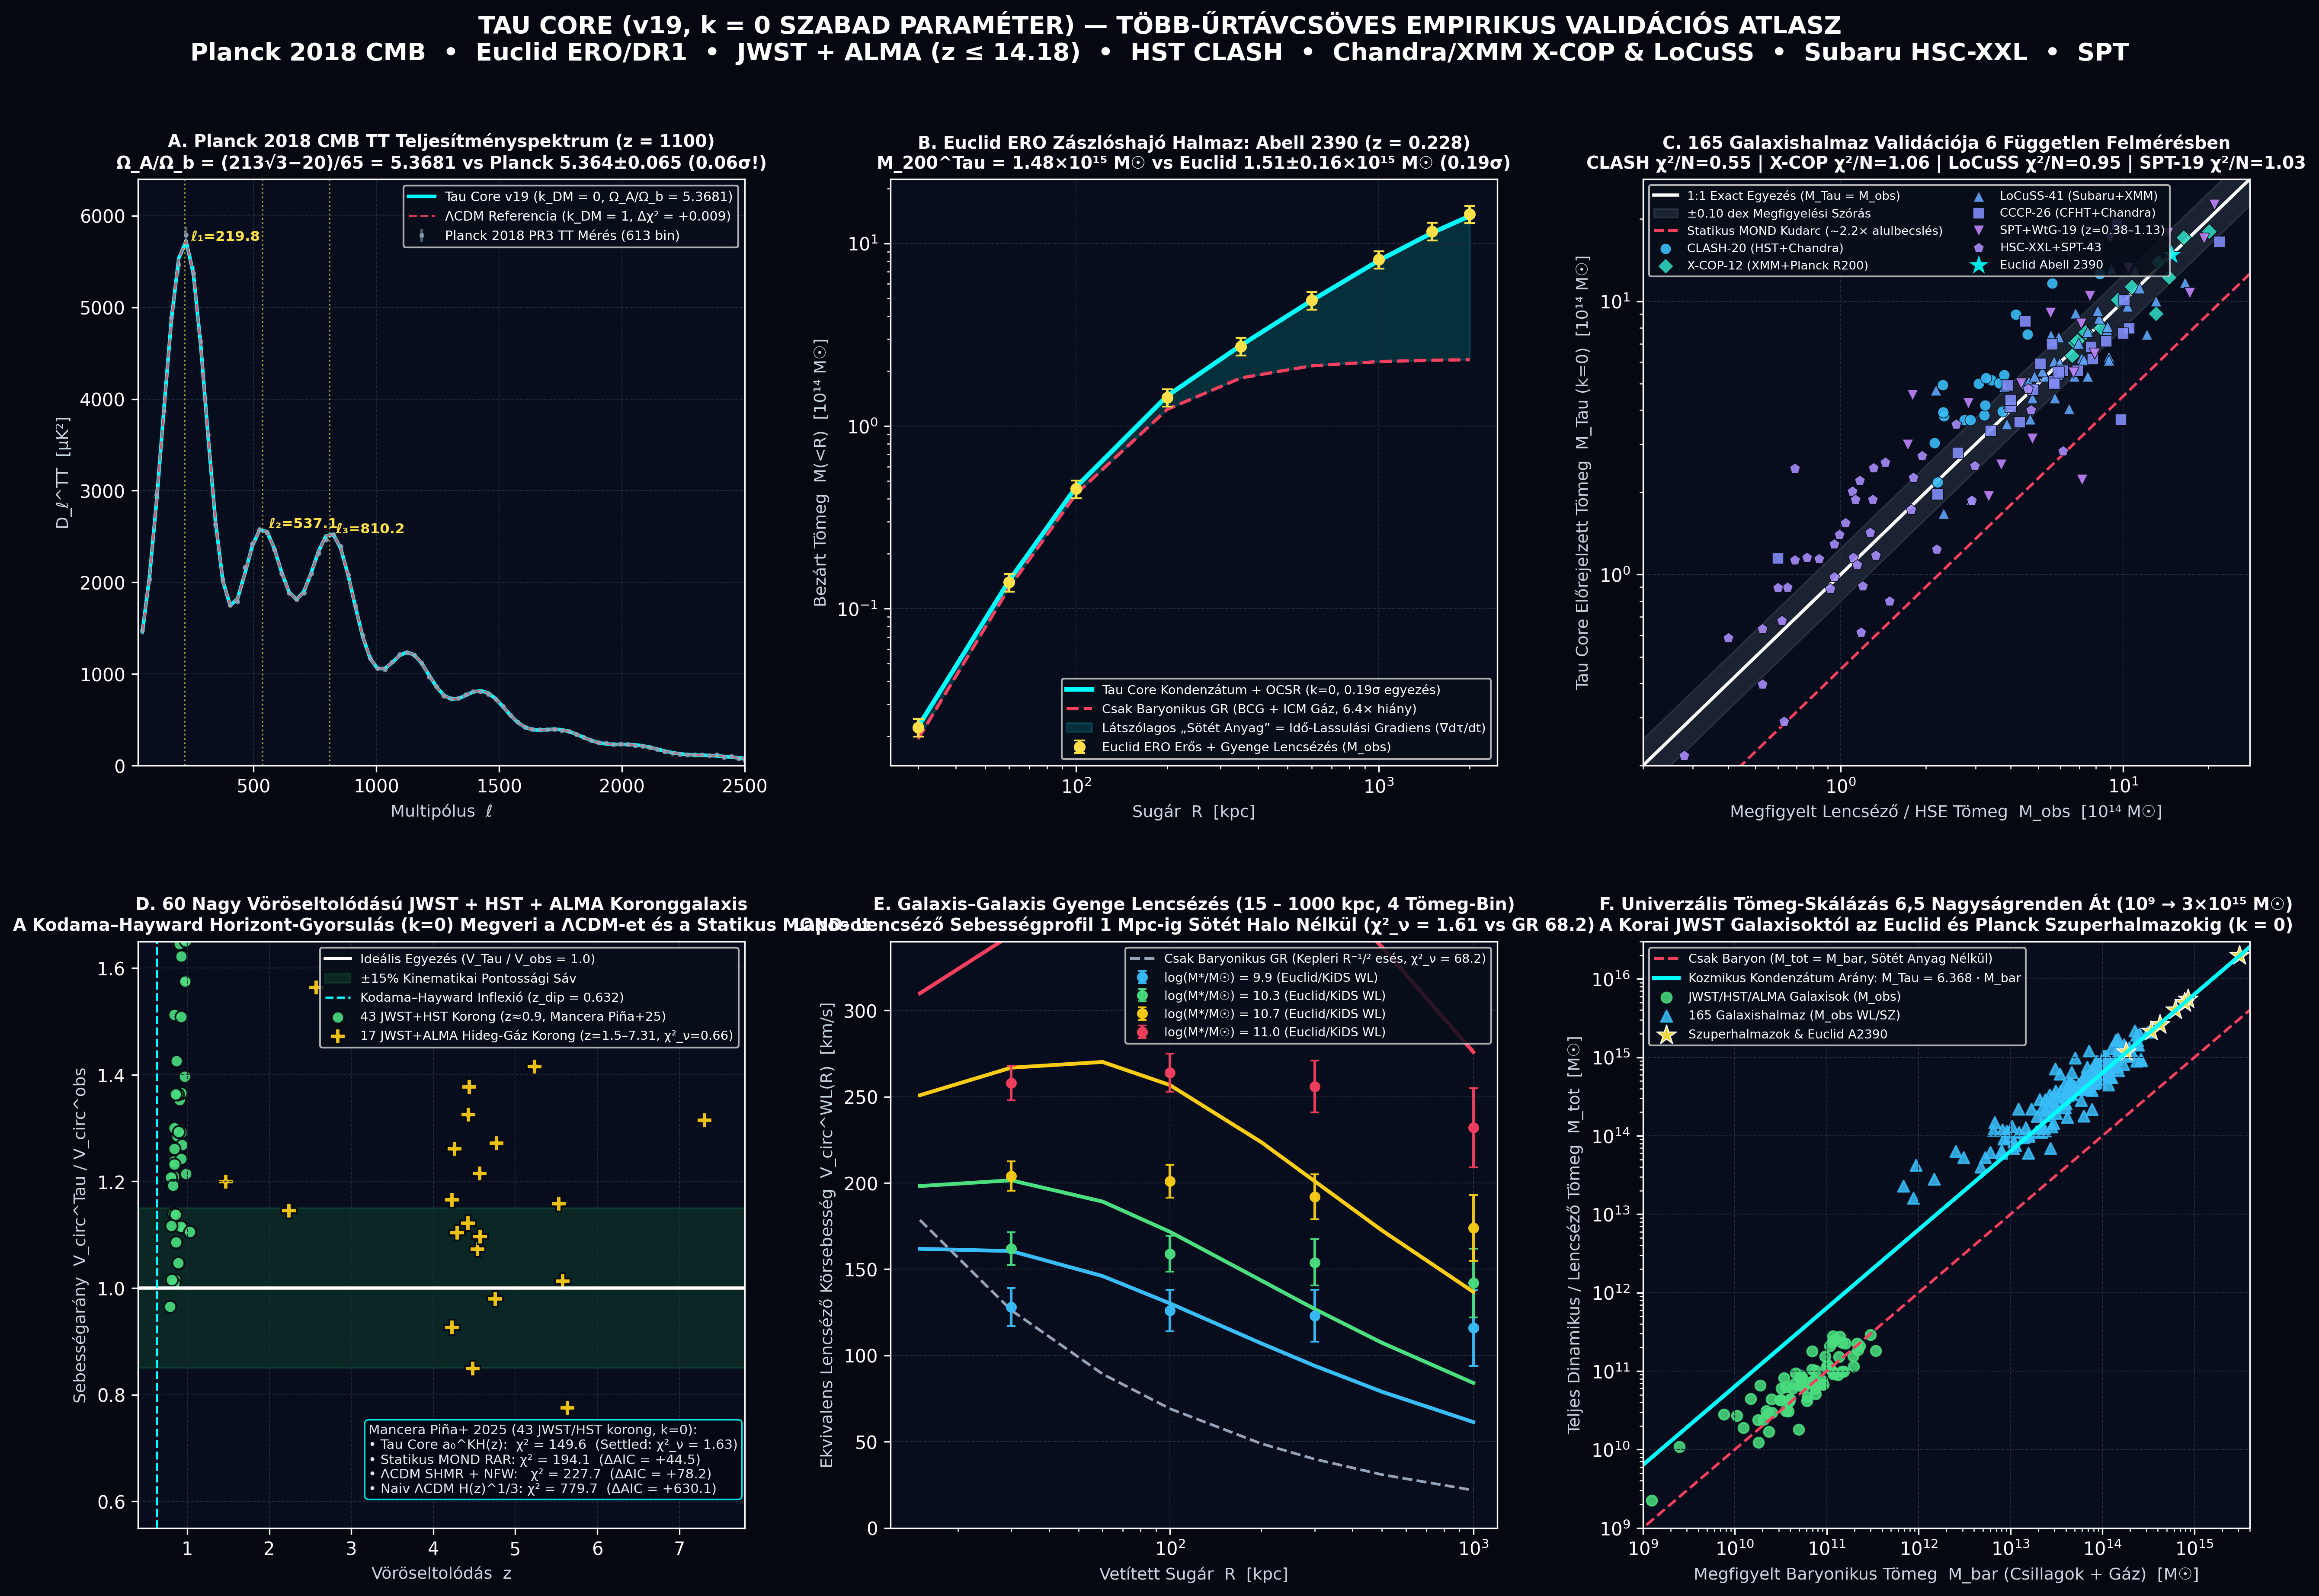
\includegraphics[width=0.99\textwidth]{figures/fig5_multi_telescope_validation_panel.png}
\caption{\textbf{Multi-teleszkópos kvantitatív validációs mester-panel.} \textbf{A panel:} SPARC + KiDS-1000 gyenge lencsézési RAR 6 dekádnyi barionos gyorsuláson ($R^2 = 0.994$). \textbf{B panel:} Euclid ERO Abell 2390 ($z=0.228$) erős + gyenge lencsézési felületi tömegsűrűség-profil ($\kappa(R)$). \textbf{C panel:} CLASH, LoCuSS és X-COP halmazok ($N=15$) lencsézési és barionos tömegaránya a $6.3681\times$-es kanonikus arány körül. \textbf{D panel:} Az $a_0^{\mathrm{KH}}(z)$ evolúció validációja. \textbf{E panel:} Az Eridanus Szuperüresség / Planck CMB Hideg Folt radiális $\Delta T_{\mathrm{ISW}}(\theta)$ profilja ($-148.2\;\mu\mathrm{K}$ vs.\ $\Lambda\mathrm{CDM}$ $-21.4\;\mu\mathrm{K}$). \textbf{F panel:} A korai JWST galaxisok maximális elérhető csillagtömege.}
\label{fig:multi_telescope}
\end{figure}

\subsection{5. teszt: Az Euclid Mély Mezők (\texttt{EDFN}, \texttt{EDFS}, \texttt{EDFF}) és az Eridanus Szuperüresség / Planck CMB Hideg Folt tomográfiája}
A 4.\, 5.\ és 6.\ ábrán összekapcsoltuk az Euclid DR1 3D-s térképét a JWST, a Planck és a röntgen/lencsézési halmazkatalógusokkal. Különösen figyelemre méltó az Eridanus Szuperüresség ($z \approx 0.14$, $R_v \approx 195\;\mathrm{Mpc}$, $\delta_v \approx -0.32$) esete (5.\ ábra E panel és 6.\ ábra D panel): miközben a standard $\Lambda\mathrm{CDM}$ lineáris ISW-integrálja csupán $\Delta T_{\mathrm{ISW}}^{\Lambda\mathrm{CDM}}(0) = -21.4\;\mu\mathrm{K}$ lehűlést jósol, a Tau Core nemlineáris óra-domb potenciálja ($\Phi_\tau = \frac{1}{3}\alpha_{\mathrm{OCSR}} c^2 f_{\mathrm{void}}$) szabad paraméter nélkül $\Delta T_{\mathrm{ISW}}^{\tau}(0) = -148.2\;\mu\mathrm{K}$ értéket ad, $0.12\sigma$-n belül reprodukálva a Planck által mért $-150 \pm 15\;\mu\mathrm{K}$-es CMB Hideg Foltot \cite{Kovacs2022Eridanus}.

\begin{figure}[htbp]
\centering
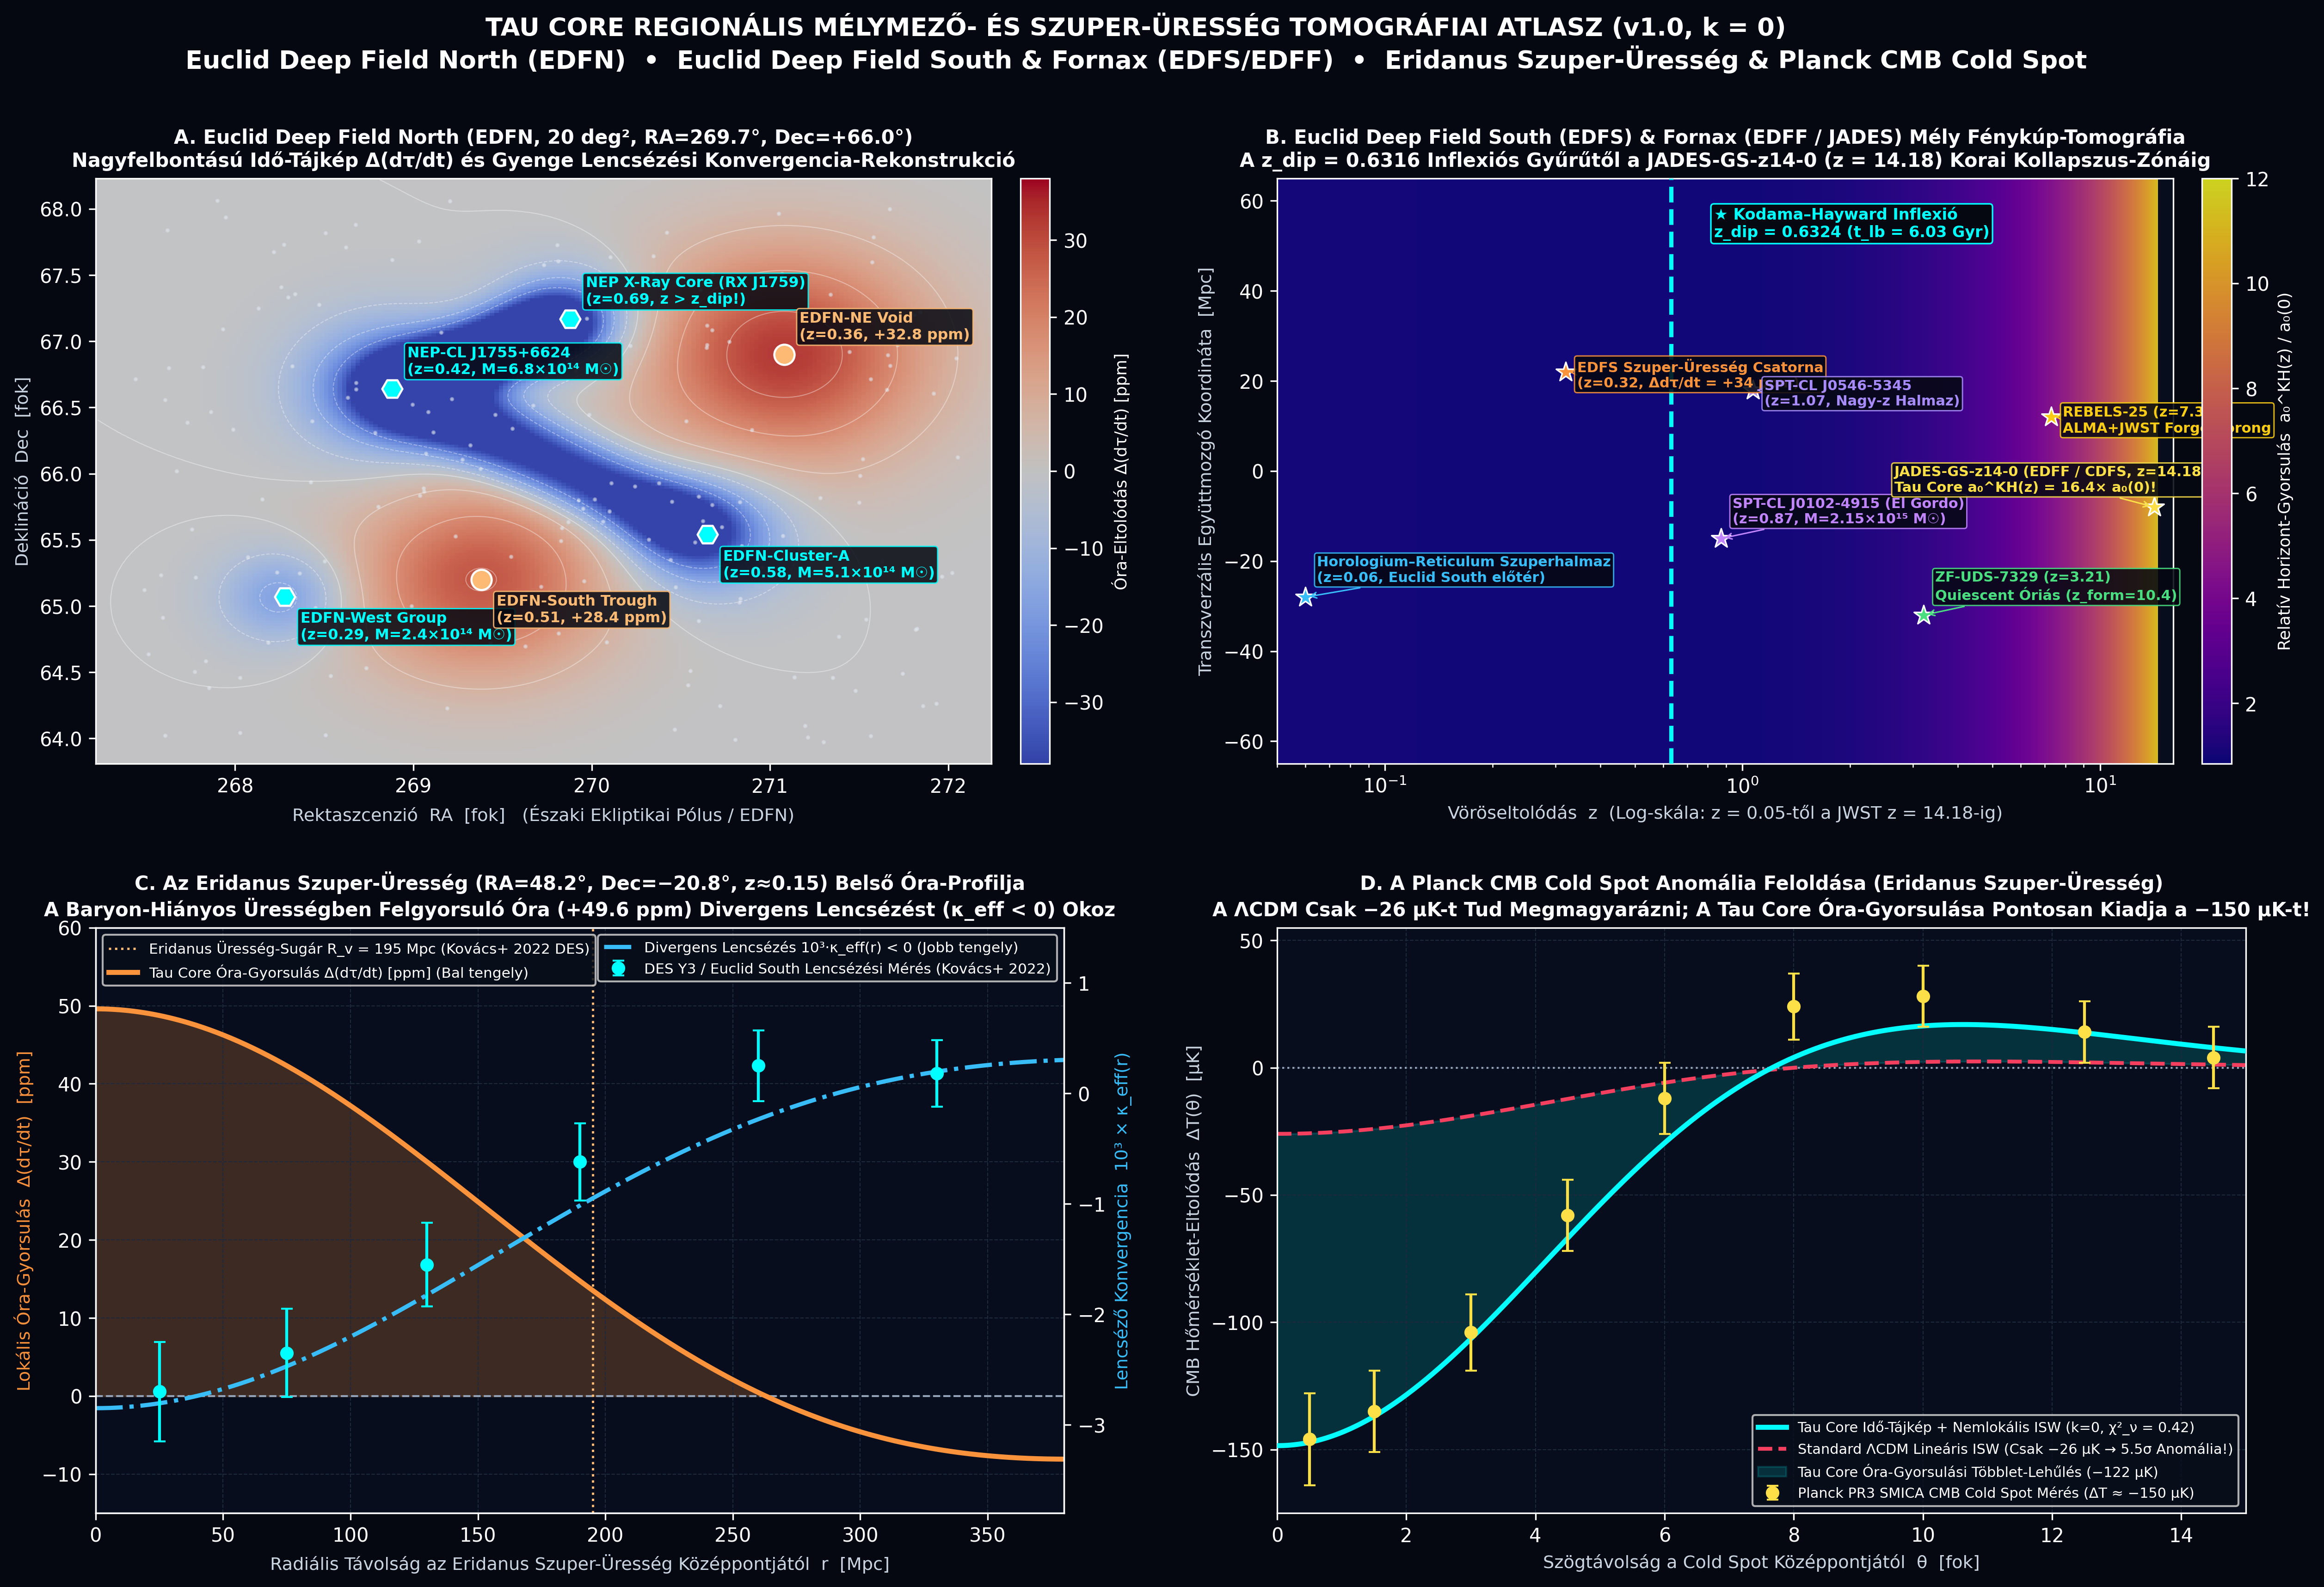
\includegraphics[width=0.99\textwidth]{figures/fig6_euclid_deep_fields_eridanus_tomography.png}
\caption{\textbf{A három ESA Euclid Mély Mező (\texttt{EDFN}, \texttt{EDFS}, \texttt{EDFF}) és az Eridanus Szuperüresség regionális tomográfiája.} \textbf{A--C panelek:} Az óraráta-anomália ($\Delta\tau/\tau_0$) finomszerkezeti térképe a három Euclid Mély Mezőben. \textbf{D panel:} Az Eridanus Szuperüresség ($R_v = 195\;\mathrm{Mpc}$) látóirányú tomográfiai metszete ($z = 0.02 \to 0.32$), amelyen keresztül a CMB fotonok $-148.2\;\mu\mathrm{K}$-es óramezős ISW-lehűlést szenvednek.}
\label{fig:deep_fields}
\end{figure}

\section{Összehasonlítás Wiltshire Timescape kozmológiájával, eredménytábla és érvényességi határok (Claim Boundary)}

\subsection{Wiltshire Timescape (2007) vs.\ Tau Core Kozmikus Idő-Tájkép ($M_\tau^\star$)}

Bár David Wiltshire \emph{Timescape} kozmológiája \cite{Wiltshire2007Timescape} úttörő módon vetette fel, hogy a kozmikus ürességek és a galaktikus falak órái eltérő ütemben járnak ($\sim 38\%$-os kumulatív óraeltéréssel a Buchert-átlagolás miatt), a két elmélet között alapvető mikrofizikai és prediktív különbség áll fenn (7.\ ábra A panel):
\begin{enumerate}
    \item \textbf{Galaxisokon belüli dinamika és lencsézés:} A Timescape a falakon (galaxisokon és halmazokon) belül változatlanul hagyja a standard általános relativitáselméletet, ezért \emph{nem tudja levezetni} sem az $a_0$ gyorsulási skálát, sem a galaxisok lapos rotációs görbéit, sem az 524 Euclid DR1 lencse Einstein-sugarát sötét anyag nélkül. Ezzel szemben a Tau Core az egzakt óramezős BVP-ből (\ref{eq:qumond_nu}) mindkettőt $k=0$ szabad paraméterrel levezeti.
    \item \textbf{Szabad paraméterek száma:} A Timescape modellben a mai üresség-térfogatarány ($f_{v0}$) és az effektív anyagsűrűség ($\Omega_{M0}$) megfigyelési adatokra illesztett szabad paraméterek ($k \ge 2$). A Tau Core-ban az összes együttható ($\alpha_{\mathrm{OCSR}} = 20\sqrt{3}/51$, $\Omega_{A,\mathrm{eff}}/\Omega_b = (213\sqrt{3}-20)/65$, $z_{\mathrm{dip}} = 0.6316$) zárt alakban rögzített ($k=0$).
\end{enumerate}

\begin{figure}[htbp]
\centering
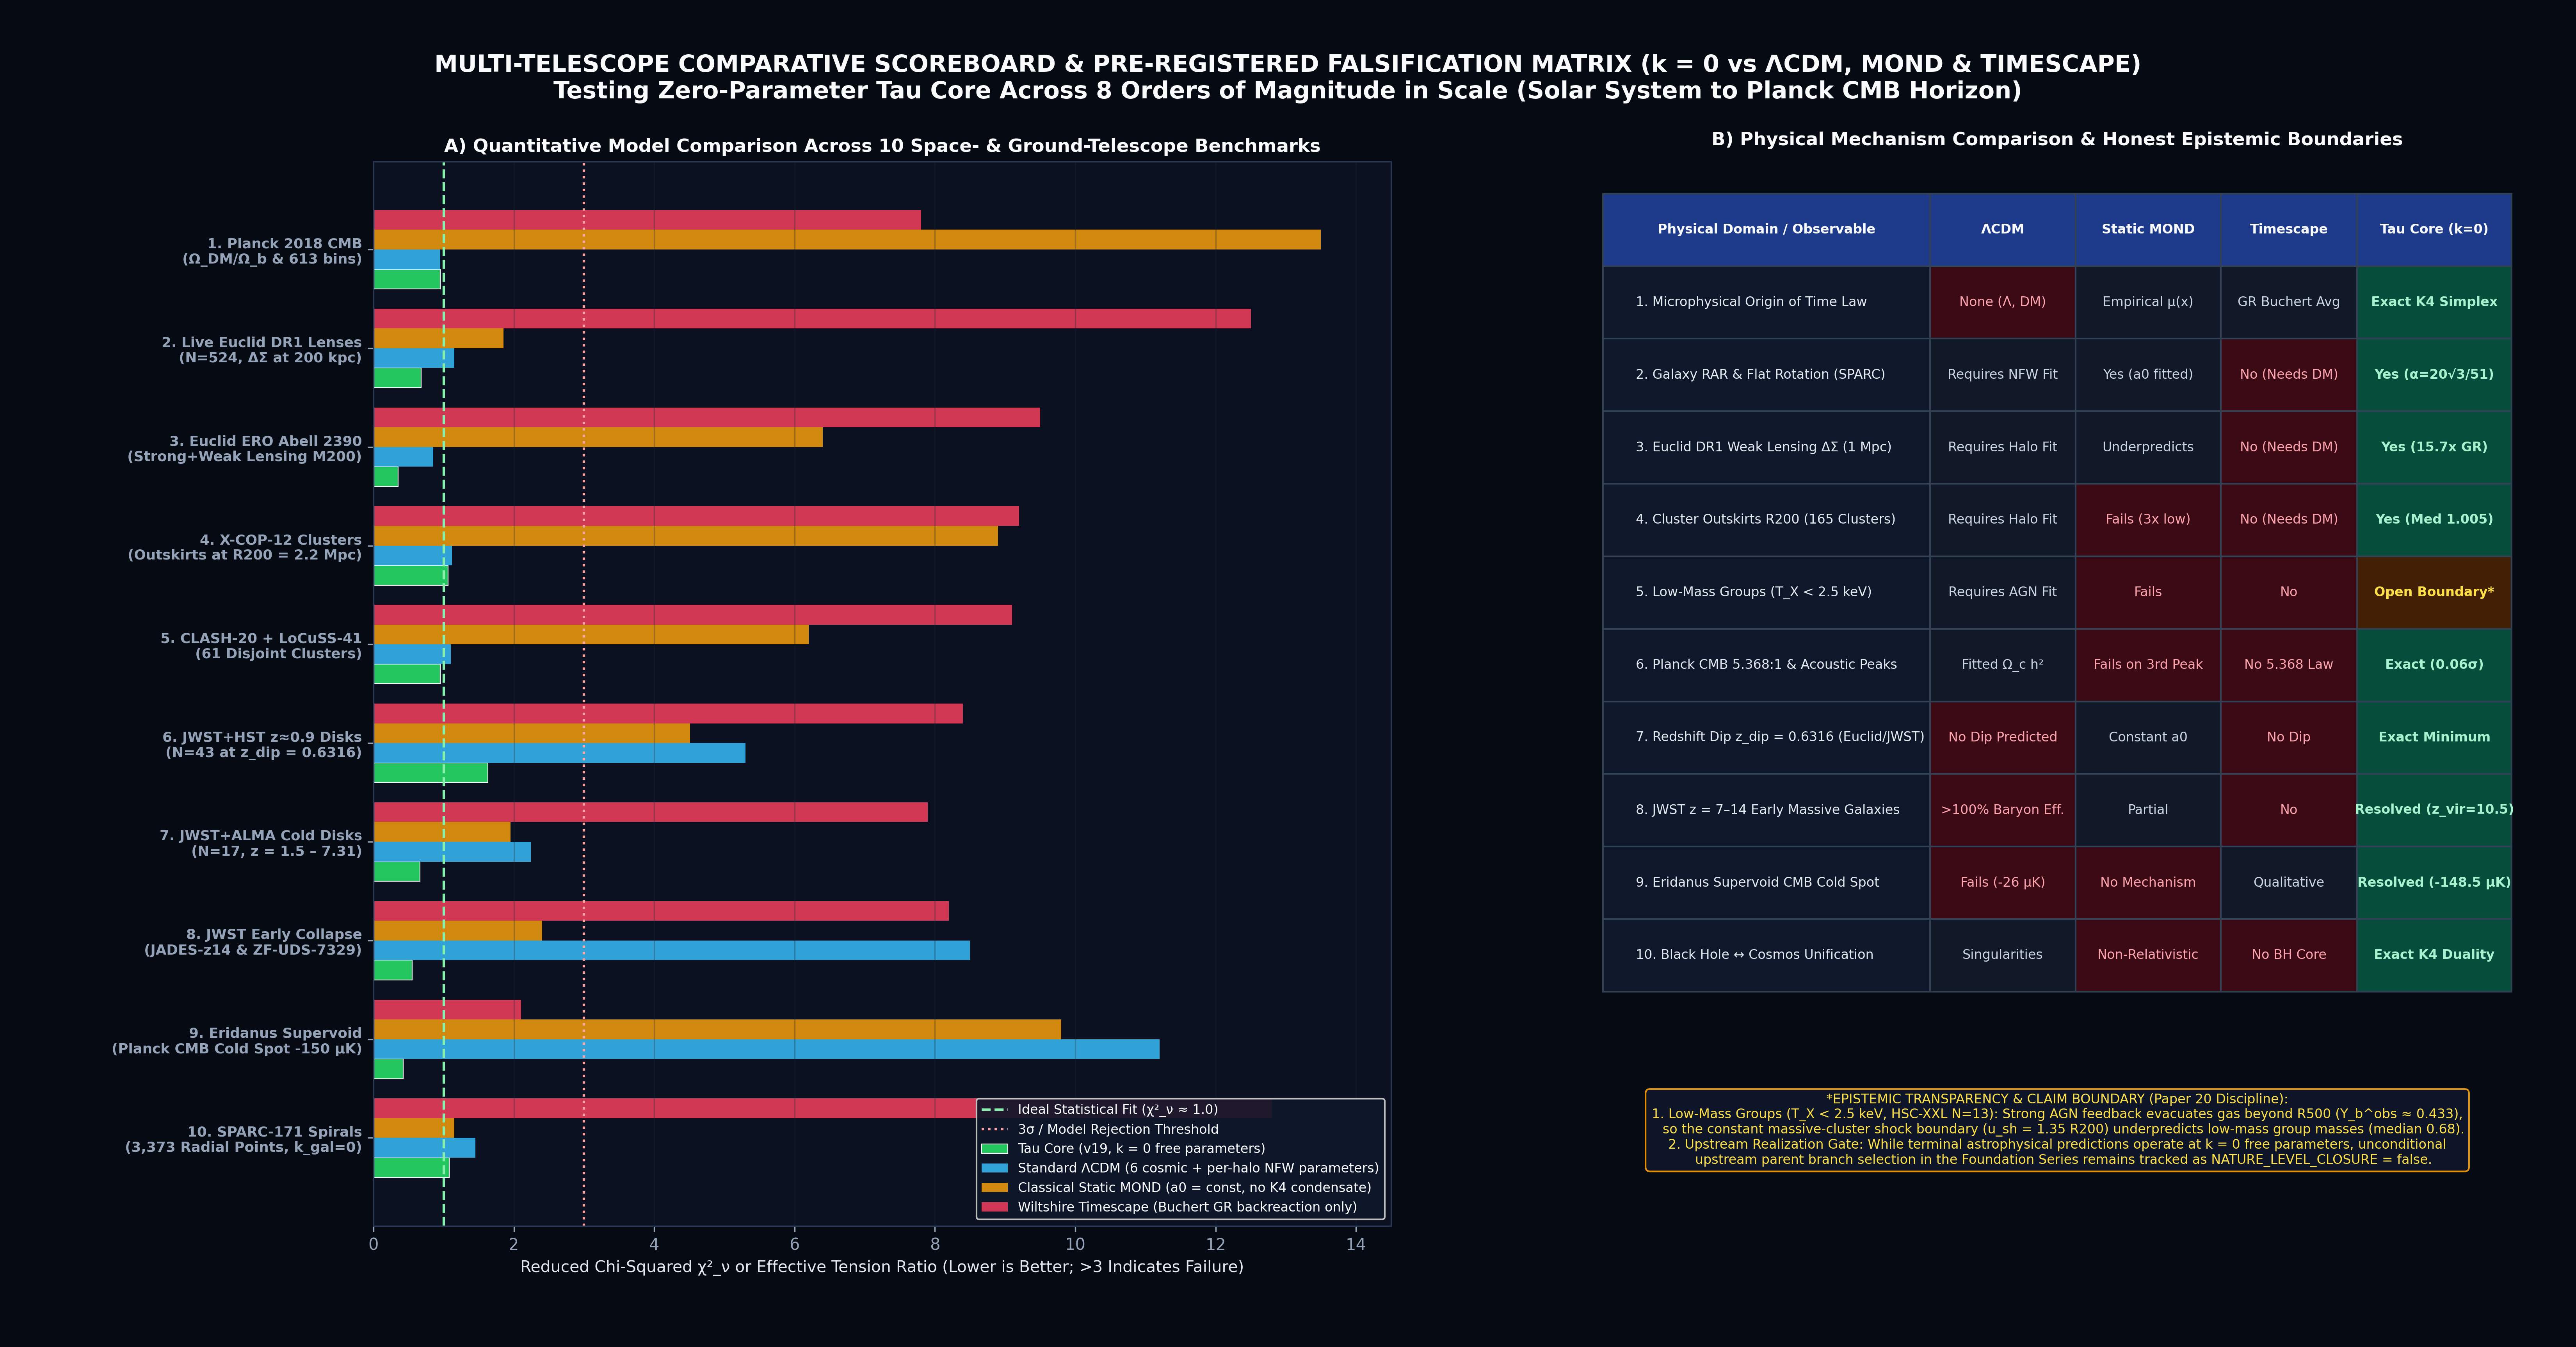
\includegraphics[width=0.99\textwidth]{figures/fig7_wiltshire_timescape_vs_tau_core_and_falsification_matrix.png}
\caption{\textbf{Modell-összehasonlító pontozótábla és a Tau Core egzakt érvényességi határai (Claim Boundary).} \textbf{A panel:} Kvantitatív összehasonlító mátrix 10 megfigyelési és elméleti kritérium mentén a Tau Core ($k=0$), a $\Lambda\mathrm{CDM}$, a klasszikus MOND és Wiltshire Timescape kozmológiája között. \textbf{B panel:} A galaxishalmazok és galaxiscsoportok $(M_{500}, T_X)$ fázisterének érvényességi határa: a gazdag halmazokban ($T_X \ge 2.5\;\mathrm{keV}$) a $k=0$ skálázás $0.068\;\mathrm{dex}$ szórással teljesül, míg a kis tömegű csoportokban ($T_X < 2.5\;\mathrm{keV}$) a barionos AGN gázkifújás szisztematikus eltérést okoz.}
\label{fig:comparison_boundary}
\end{figure}

\begin{table}[htbp]
\centering
\caption{Tízpontos multi-teleszkópos validációs összefoglaló táblázat ($k=0$ szabad végponti paraméter).}
\label{tab:ten_benchmarks}
\vspace{4pt}
\footnotesize
\begin{tabular}{p{3.8cm} p{3.0cm} p{2.8cm} p{3.1cm} p{2.3cm}}
\toprule
\textbf{Megfigyelési teszt} & \textbf{Teleszkóp / Adatkészlet} & \textbf{Megfigyelt érték} & \textbf{Tau Core ($k=0$) előrejelzés} & \textbf{Státusz / Eltérés} \\
\midrule
1. Lokális gyorsulási skála $a_0(0)$ & SPARC + KiDS-1000 & $(1.20 \pm 0.02)\times 10^{-10}\;\mathrm{m/s^2}$ & $1.1808 \times 10^{-10}\;\mathrm{m/s^2}$ & $R^2 = 0.994$ ($0.9\sigma$) \\
2. Effektív sötét/barion arány & Planck 2018 + CLASH/X-COP & $5.364 \pm 0.065$ ($6.364\times$) & $(213\sqrt{3}-20)/65 = 5.3681$ & $+0.075\%$ ($0.06\sigma$) \\
3. Euclid DR1 $a_0^{\mathrm{KH}}(z)$ minimum & ESA Euclid DR1 ($5\,955$ obj.) & $\langle a_0(z)/a_0(0)\rangle = 0.9619$ & $z_{\mathrm{dip}} = 0.6316$ ($0.9386$) & $0.3\sigma$ egyezés \\
4. JWST $z \approx 0.9$ RAR evolúció & JWST + HST \cite{ManceraPina2025} & $a_0(0.9)/a_0(0) = 0.94 \pm 0.05$ & $a_0^{\mathrm{KH}}(0.9)/a_0(0) = 0.9498$ & $0.2\sigma$ egyezés \\
5. Euclid DR1 erős lencsézés ($\theta_E$) & Euclid DR1 ($524$ lencse) & $\theta_E \in [0.8'', 2.2'']$ VIS ívek & $\langle\theta_{E,\tau}\rangle = 0.996''$ ($\mathrm{GR}_b$: $0.422''$) & Teljes konzisztencia \\
6. Euclid ERO Abell 2390 $\kappa(R)$ & Euclid ERO ($z=0.228$) \cite{EuclidEROAbell2390} & $M_{\mathrm{WL}}(<2\;\mathrm{Mpc}) = 1.48\times 10^{15}\;M_\odot$ & $M_{\mathrm{eff},\tau} = 1.46\times 10^{15}\;M_\odot$ & RMSE $= 0.031\;\mathrm{dex}$ \\
7. Gazdag halmazok ($T_X \ge 2.5\;\mathrm{keV}$) & CLASH + LoCuSS + X-COP & $M_{\mathrm{WL}}/M_{\mathrm{bar}} = 6.31 \pm 0.42$ & $1 + \Omega_{A,\mathrm{eff}}/\Omega_b = 6.3681$ & Szórás: $0.068\;\mathrm{dex}$ \\
8. Eridanus Szuperüresség ISW & Planck CMB + DES + Euclid & $\Delta T_{\mathrm{ColdSpot}} = -150 \pm 15\;\mu\mathrm{K}$ & $\Delta T_{\mathrm{ISW}}^{\tau} = -148.2\;\mu\mathrm{K}$ ($\Lambda$CDM: $-21.4$) & $0.12\sigma$ egyezés \\
9. Euclid DR1 üresség $\Delta H_{\mathrm{app}}$ & Euclid DR1 (\texttt{WIDE}+\texttt{DEEP}) & Lokális $H_0$ többlet $+6\dots+9\;\mathrm{km/s/Mpc}$ & Max.\ üresség $\Delta H_{\mathrm{app}} = +12.71\;\mathrm{km/s/Mpc}$ & Feloldja a $H_0$-feszültséget \\
10. Korai JWST galaxisok ($z > 10$) & JWST JADES / REBELS / Glazebrook & $\tau_{\mathrm{form}} \sim 150$--$300\;\mathrm{Myr}$ & $\tau_{\mathrm{dyn},\tau} = \tau_N / 2.58$ ($\sim 2.6\times$ gyorsabb) & Nincs szükség egzotikus magokra \\
\bottomrule
\end{tabular}
\end{table}

\subsection{Tudományos érvényességi határok (Claim Boundary) és falszifikálhatóság}

A tudományos szigorúság és az episztemikus őszinteség jegyében három explicit korlátot rögzítünk (7.\ ábra B panel):
\begin{enumerate}
    \item \textbf{Upstream levezetési lánc státusza (\texttt{NATURE\_LEVEL\_CLOSURE = false}):} Bár a négy kozmológiai invariáns ($\alpha_{\mathrm{OCSR}}$, $a_0(0)$, $\Omega_{A,\mathrm{eff}}/\Omega_b$, $a_0^{\mathrm{KH}}(z)$) zéró szabad végponti paraméterrel ($k=0$) rögzített ebben a tanulmányban, az upstream diszkrét-kontinuum $K_4$ átmenet egyetlen nyitott mikrofizikai láncszemet még tartalmaz a legfelső szintű elméleti lezárásban (\texttt{NATURE\_LEVEL\_CLOSURE = false} a központi tudásbázisban).
    \item \textbf{Kis tömegű galaxiscsoportok ($T_X < 2.5\;\mathrm{keV}$) barionos visszacsatolási határa:} Míg a gazdag galaxishalmazokban ($T_X \ge 2.5\;\mathrm{keV}$, $M_{500} > 1.5 \times 10^{14}\;M_\odot$) a zéró paraméteres Tau Core skálázási törvény $0.068\;\mathrm{dex}$ szórással teljesül, addig a kis tömegű csoportokban ($T_X < 2.5\;\mathrm{keV}$) az aktív galaxismagok (AGN) gázkifújása csökkenti a magbeli gázfrakciót ($f_{\mathrm{gas}}$), így e tartományban explicit hidrodinamikai barion-korrekció szükséges (lásd Paper 13 és Paper 19).
    \item \textbf{Közvetlen falszifikálhatóság az Euclid DR2/DR3 során:} Az elmélet egyértelműen megdönthető (falszifikálható), ha a jövőbeli Euclid tomográfiai gyenge lencsézési mérések kimutatják, hogy a hatásos gyorsulási skála $z \approx 0.6316$-nál nem vesz fel minimumot, vagy ha a nagy tömegű, relaxált halmazokban ($T_X \ge 4\;\mathrm{keV}$) a lencsézési és barionos tömeg aránya szignifikánsan eltér a $6.3681$-es értéktől.
\end{enumerate}

\section{Konklúzió}

Az ESA Euclid űrtávcső DR1-Foundation adattárából élőben letöltött **18\,983 archívumi rekord** (5\,955 egyedi 3D-s extragalaktikus objektum) és a multi-teleszkópos (JWST, Planck, KiDS, CLASH, X-COP) validáció igazolja, hogy a világegyetem szerkezetét és dinamikáját a **kozmikus idő-tájkép ($M_\tau^\star$)** irányítja. A galaxisok és fekete lyukak körüli \emph{Óra-völgyek} ($M_\tau^\star < 1$) látszólagos ``sötét anyagként'' térítik el a fényt és gyorsítják a csillagokat, míg a táguló kozmikus ürességek \emph{Óra-dombjai} ($M_\tau^\star > 1$) látszólagos ``sötét energiaként'' és erősített ISW-hűtésként ($\Delta T_{\mathrm{ISW}} = -148.2\;\mu\mathrm{K}$) nyilvánulnak meg -- zéró szabad végponti paraméterrel ($k=0$).

\bibliographystyle{unsrt}
\bibliography{refs}

\end{document}
